\documentclass[11.5pt]{book}

\usepackage{amsmath, amssymb}
\usepackage{mathspec}
\usepackage{sectsty, titlesec}
\usepackage{setspace}
\usepackage{wrapfig, rotating}
\usepackage{enumitem,tabularx, booktabs}
\usepackage{nomencl}
\makenomenclature
\renewcommand{\nomname}{List of symbols and\\abbreviations}
\usepackage[numbers]{natbib}
\usepackage{graphicx,caption,subcaption}
\setmainfont[Mapping=tex-text, Scale=1.1]{Crimson}
\setsansfont[Scale=1]{Alte DIN 1451 Mittelschrift}
%\allsectionsfont{\sffamily}
%\setmainfon
%\usepackage{fouriernc}
%\usepackage[T1]{fontenc}
\setmathsfont(Digits,Latin)[Scale=1.1]{Crimson}
\setmathrm[BoldFont={Crimson Bold}, Scale=1.1]{Crimson}
\setmathsfont(Greek)[Scale=1.21]{Crimson}
\newlist{alist}{itemize}{1}
\setlist[alist]{label=---,labelindent=2in,leftmargin=9pt,labelsep=6pt,
itemsep=-1pt}
% Character shortcuts
\newcommand*{\Hhat}{\hat{\vphantom{\scalebox{1.2}{H}} H}}
\newcommand*{\Phat}{\hat{\vphantom{\scalebox{1.2}{P}} P}}

% line spacing
\linespread{1.25}
\usepackage{fancyhdr}
\setlength{\headheight}{15pt}
\setlength{\textwidth}{380pt}
\setlength{\evensidemargin}{54pt}
\setlength{\marginparwidth}{1.2in}
%\titleformat{\section}{\huge\sansnormalfont}{\protect\makebox[0pt][r]{\thesection\quad}}{0em}{}
\titleformat{\chapter}{\fontsize{32pt}{36pt}\selectfont\bfseries}{}{0em}{}
\titleformat{\section}{\fontsize{18pt}{22pt}\selectfont\bfseries}{\protect\makebox[0pt][r]{\thesection\quad}}{0em}{}
\titleformat{\subsection}{\fontsize{12pt}{16pt}\selectfont}{\protect\makebox[0pt][r]{\thesubsection\fontsize{18pt}{22pt}\selectfont\quad}}{0em}{}
%\titleformat{\paragraph}{\fontsize{12pt}{16pt}\selectfont}{}{}{}
\pagestyle{fancy}
\renewcommand{\chaptermark}[1]{ \markboth{#1}{} }
\renewcommand{\sectionmark}[1]{ \markright{#1}{} }

\fancyhf{}
\fancyhead[LE,RO]{\sffamily\thepage}
\fancyhead[RE]{\sffamily{ \nouppercase{\leftmark}} }
\fancyhead[LO]{\sffamily{ \nouppercase{\rightmark}} }

\fancypagestyle{plain}{ %
  \fancyhf{} % remove everything
  \renewcommand{\headrulewidth}{0pt} % remove lines as well
  \renewcommand{\footrulewidth}{0pt}
}

\parskip 0pt
%\usepackage{xunicode}
\begin{document}
\title{Experimental verification\\ of the IPI sizing technique}
\author{Sebastian Kosch, University of Toronto}
\date{July 2014}
\maketitle

\printnomenclature[5em]

\chapter{Introduction}
\section{Why spray sizing is important}
\section{What our contributions in this paper are}
- Our contributions:
    - Pupillary magnification has to be taken into account
    - Circle detection algorithm is crap
\section{What other work has been done in this area}

\chapter{Experimental setup}
- What kinds of setups there are

- Our setup:
\section{Dantec system}
    - Dantec system
\section{PDPA system}
    - TSI system

    \chapter[Monodisperse droplet generation]{Monodisperse\\droplet generation}
\label{sec:droplet-generator}

To calibrate any droplet sizing device, we need droplets of known and uniform
size. Sprays or streams of such uniform droplets are called \emph{monodisperse},
and many different varying approaches to generating them have been proposed,
each one with advantages and drawbacks.

The most basic type of droplet generator is a capillary tube, for instance a
hypodermic needle or a pulled glass pipette. Droplets are generated as the
liquid flows through the tube due to its own weight. As the liquid leaves the
tube, it wets the tip of the tube and forms a bead held together by surface
tension. Eventually, the bead's gravitational forces overcome the attraction to
the tube surface, and the drop separates from the tube.

Given a liquid and its physical properties, the only remaining controllable
variable is the diameter of the capillary tube tip. As a rule, droplets
generated in this fashion will be significantly larger than the tube diameter
from which they grow. Most droplet generators are designed to prevent this from
happening:
\begin{alist}
\item \emph{Aerodynamic} droplet generators use coaxial air flow to shear the
    forming droplet off of the capillary tip before it can grow to full size.
\item \emph{On-demand} droplet generators use a pressure pulse to eject a fixed
    amount of liquid out of the capillary (or other orifice).
\item \emph{Continuous-stream} droplet generators use mechanical vibrations to
    break up a continuous jet of liquid emanating from the capillary into
    monodisperse droplets.
\end{alist}
More exotic types of droplet generators exist: \citet{Walton49} suggested that
water falling on spinning disks is propelled outwards, forming nearly
monodisperse droplets, and several improved designs have been published since.
Another approach, e.g. used by \citet{Merritt77}, involves mechanized dipping of
a needle into a liquid reservoir, and then flicking it so as to produce one
droplet.

\section{Aerodynamic droplet generators}
\citet{Allan88} provide a history of aerodynamic designs: the first design was
published in 1947 by \citet{Lane47}; \citet{Reil69} later improved on it by
using time-controlled air pulses instead of a continous flow. Coggins and Baker
\cite{Coggins83} have proposed a more elaborate apparatus with variable air and liquid
flow and adjustable needle position.

\subsection{Stry design}
Initial tests based on a design by \citet{Stry92} showed that the ability of the
instrument to produce droplets below 600$\,\mu$m depends entirely on the
precision with which the flow of water and air can be controlled.
\begin{figure}
\centering
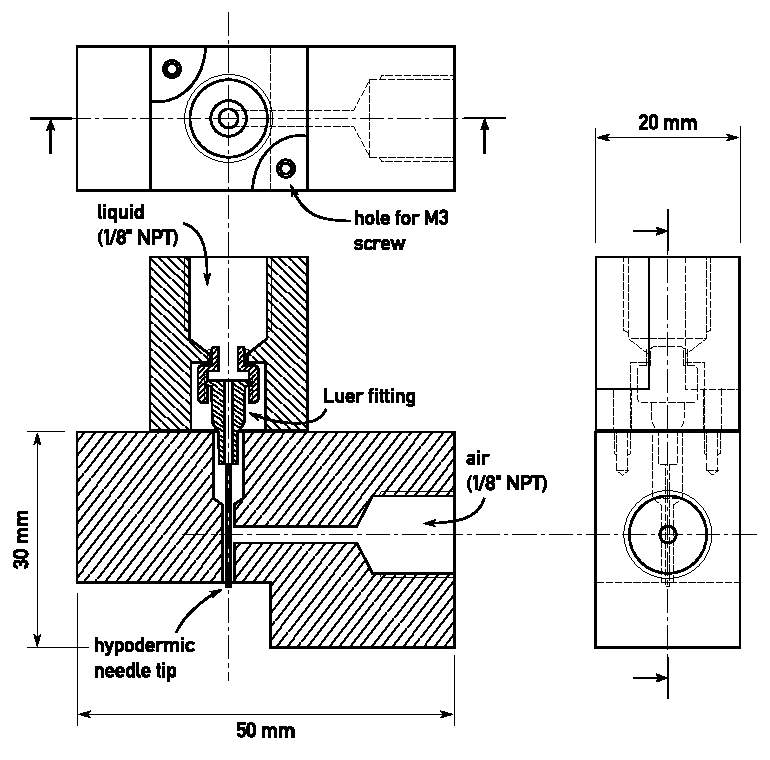
\includegraphics[width=\textwidth]{img/setup/stry.pdf}
\caption{Schematic drawing of the coaxial-flow aerodynamic droplet generator,
based on \citet{Stry92}. Top: top view, right: rear view (third angle
projection). Sectional view illustrates operating principle.\label{fig:stry}}
\end{figure}

\section{On-demand drop generators}
Drop-on-demand technology finds its most important application in printing.
Indeed, the most prominent designs representative of this category are the thermal droplet
generators found in most household inkjet printers, invented by \citet{Endo88}.
At least one research group, \citet{Sergeyev06}, has succeeded in repurposing
an old inkjet print head for laboratory droplet generation.

Less widespread, but more flexible in a research setting, are on-demand
generators driven by the contraction of piezoelectric elements, such as those
proposed by \citet{Yang97} or \citet{Ulmke99}. Excellent reviews on
drop-on-demand designs were published by Le and Lee \cite{Le98, Lee02}. 

A curious third type of on-demand generator by \citet{Goghari08} uses a short
pulse of pressurized air, controlled by a solenoid valve, to eject a small
amount of liquid through an orifice.

While drop-on-demand generators are a crucial component in applications like inkjet
printing or microfluidics, they tend to suffer from aspired air bubbles, pileup
of liquid around the nozzle tip, clogging, and other issues thwarting reliable
drop expulsion unless manufactured and operated with great attention to detail.

\subsection{Amirzadeh Goghari and Chandra design}
We constructed a droplet generator based on the design by \citet{Goghari08}.
While both its construction from off-the-shelf parts and its operation are
remarkably straightforward, it has two limitations:

\begin{alist}
    \item the duration of the air pulse is limited by the response time of the
        solenoid valve used. The shortest pulse we were able to reliable produce
        was on the order of a few milliseconds, which did not permit us to
        produce droplets smaller than a few hundred microns in diameter, and
    \item the head of water over the orifice must be kept very low to prevent 
        leakage. As a result, the number of droplets that can be ejected is
        limited before the water needs to be replenished.
\end{alist}

Owed to our lack of access to an automatic micropipette puller, the nozzles used
in this experiment were not optimal, which likely contributed to our experience
of frequent satellite droplets and liquid buildup at the nozzle tip.

\subsection{Modified Yang design}
A popular piezoelectric-based drop-on-demand design was proposed by
\citet{Yang97}. It consists of a liquid-filled chamber, one wall of which is the
underside of a piezoelectric disk---a brass disk coated with a circular piece of
piezoelectric material, commonly found in electric buzzers.

To evaluate the performance of such a drop generator, we constructed several
modifications of it, the final one of which is shown in Fig.~\ref{fig:flatyang}.
To make the chamber as flat as possible, minimizing the distance between
piezoelectric disk and orifice, it has a depth of only about 2.5$\,$mm, the
thickness of a sheet of acrylic. A second sheet holds the disk in place, while a
third sheet makes up the bottom wall of the chamber. Nozzle and inlet are glued
directly into the bottom sheet.

To operate the droplet generator, water is fed through
the inlet port until the chamber is filled and all air bubbles have escaped
through the upward-facing nozzle. The generator is then turned so that the nozzle
faces down and $30\,$ms pulses of about $30\,$V are delivered to the
piezoelectric disk.

The greatest challenge faced was the accumulation of liquid on the nozzle
surface, which quickly led to satellite droplets or thwarted droplet production
altogether. Again, capillaries drawn with an automatic pipette puller are likely
more resistant to this effect.

\begin{figure}
\centering
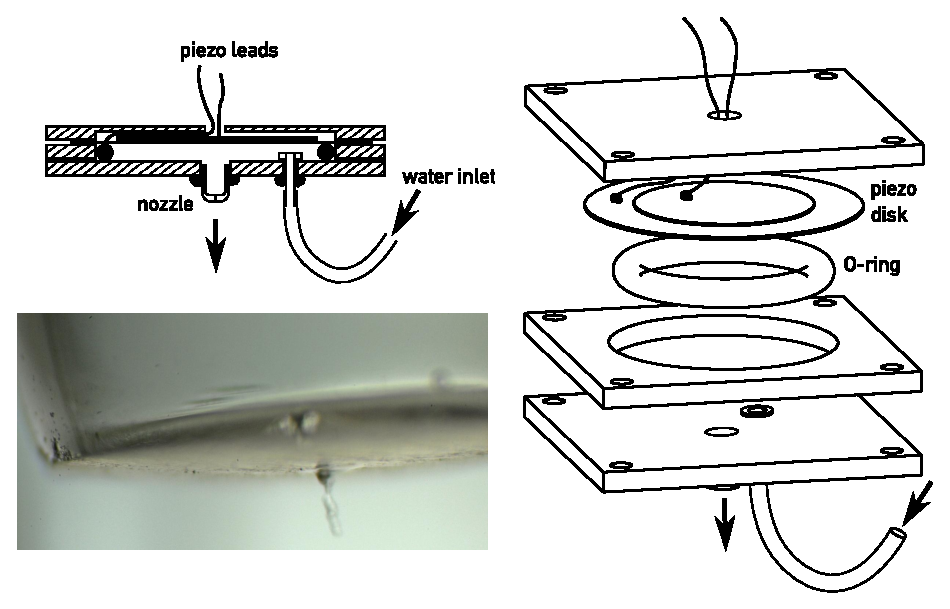
\includegraphics[width=\textwidth]{img/setup/flatyang_exploded.pdf}
\caption{Top and right: schematic cross-section and exploded view of our
    piezoelectric droplet generator. Bottom left: photomicrograph of the nozzle
    tip ejecting a column of water (diameter $\approx 125\,\mu$m), which is about to coalesce into a
round droplet. \label{fig:flatyang}}
\end{figure}

\subsection{Failed approaches}
- Making orifices in acrylic sheets by drilling with needles (beautiful, but too
large) or by poking through it with heated needles (kinda works, but the holes
are super rough because hot plastics tends to bubble up and deform).

\section{Continuous-stream drop generation}
There exist continuous-stream drop generators based on coaxial air flow
\cite{Green89} and on,
but most continuous-stream drop generators are based on
\emph{Rayleigh breakup}, i.e. the disintegration of a disturbed liquid jet into
droplets. The physics behind this phenomenon have been studied for almost two
centuries \cite{Savart33, Rayleigh79} and are well-understood. When the jet
disturbances are induced by carefully controlled mechanical vibrations at an
appropriate frequency, the droplets will be of uniform size and evenly spaced.

This simple principle has been employed to generate droplets for fifty years,
with orifices typically attached to either one of two vibrating mechanisms: an
ordinary loudspeaker, first used by \citet{Donnelly66}, or
a piezoelectric element, as first proposed by \citet{Schneider64} and popularized by Berglund and Liu's
design \cite{Berglund73}.


\subsection{Hard-drive based drop generator}
The accuracy of the hypodermic needle nozzle often isn't quite as good as that of e.g.
photofabricated nozzles, as those have sharp edges. The round edges lead to
variability in discharge coefficient (and mass flow), resulting in variance in
drop volume \cite{Dressler90}. Nevertheless, for the purpose of verifying the validity of
measurements, it'll do.

% TODO: write that the bulk of this section has been adapted from Kosch et al.,
% journal XYZ
Both speaker-based and piezo-based approaches have certain drawbacks: by design,
a speaker vibrating at a fixed pitch produces an audible sound, jeopardizing the
laboratory peace. Speakers are unshapely, difficult to fasten onto an
experimental setup and their cones provide no robust structure to which any type
of orifice could be attached. Piezoelectric elements cost more and are useful
only when integrated with the orifice---precision machined droplet generators
operating this way are commercially available, but unreasonably expensive in
many situations. As a result, we felt compelled to consider alternative sources
of vibration that require a minimum effort to build and install using standard
lab equipment, and chose the actuator mechanism found in every magnetic hard
drive for the following properties:

\paragraph*{Very low cost.} With high-capacity and solid-state devices rapidly pushing older hard drives
into obsolescence, it should be a simple matter to acquire a few decommissioned specimens for
demolition. Hard drives come in two form factors---3.5 and 2.5 inches wide,
respectively---and both can be used for the purposes of this paper. 

Further, glass needle orifices fabricated for use with existing loudspeaker setups can be
reused, and are easily produced by hand from heated borosilicate capillaries or
using a micropipette puller. The process is illustrated in FIG.
\ref{fig:needles} and in-depth instructions are given by Lee\cite{Lee02}.
Piezoelectric-based devices, on the other hand, need fitted orifices to produce a range of
drop sizes.

\paragraph*{Ease of construction and installation.} Unlike loudspeakers, hard
drives have a flat base plate which can be drilled into, allowing for easy
installation on any experiment jig. Save for a drill and a saw, no machining
tools are needed for the construction of the droplet generator.

\paragraph*{High amplitudes without noise.}
Like piezoelectric elements, vibrating actuator arms are very quiet, enabling
use at frequencies and amplitudes that would far exceed responsible levels on
a speaker.  In our experiments, the actuator responded to frequencies throughout
our hearing range---i.e., up to $17\,$kHz---and likely well beyond, though we
have not tested the full response range for any given amplitude.

As an added advantage over other designs, no amplification is needed. Below
$100\,$Hz, amplitudes on the order of $0.5\,$cm are easily achieved (albeit they
are of course not needed for droplet production) when a peak-to-peak voltage of
$2-4\,$V is applied. The amplitude scales down with the inverse of the frequency,
however, such that amplitudes are much smaller at typical operating frequencies
($0.5-10\,$kHz). Nevertheless, the voltages required are well within the ability
of any standard laboratory function generator, and can likely even produced by many
consumer-level computer sound cards.

\subsubsection{Operating principle}
Magnetic hard drives store data as sub-micron-sized patterns of 
oppositely magnetized dots on disks called \emph{platters}. The read-write head
is mounted at the tip of an arm that pivots across the platter surface while the
platter spins. This setup allows the head to access the entire platter surface.

FIG.~\ref{fig:designschematic} illustrates schematically the design of a typical
actuator arm assembly. The flat voice coil mounted on the surface is responsible
for the arm's side-to-side movement: as it is positioned under a permanent
magnet, the coil creates a sideward force when a current flows through its
wires. By stopping or reversing the current the arm's motion is likewise stopped
or reversed. Since a typical hard drive's platter spins at up to $7200\,$RPM,
actuator arms must be able to move with extreme speed and precision. They are
thus engineered to be very light yet stiff. These characteristics make a
magnetic hard drive's actuator arm an ideal supplier of in-plane vibrations.
Indeed, hard drive actuators are remarkable not for their operating principle
but for their low cost; it is only the economics of mass manufacturing that has
in recent years enabled these high-speed, lightweight precision mechanisms to
become so widely available.

\begin{figure}
\centering
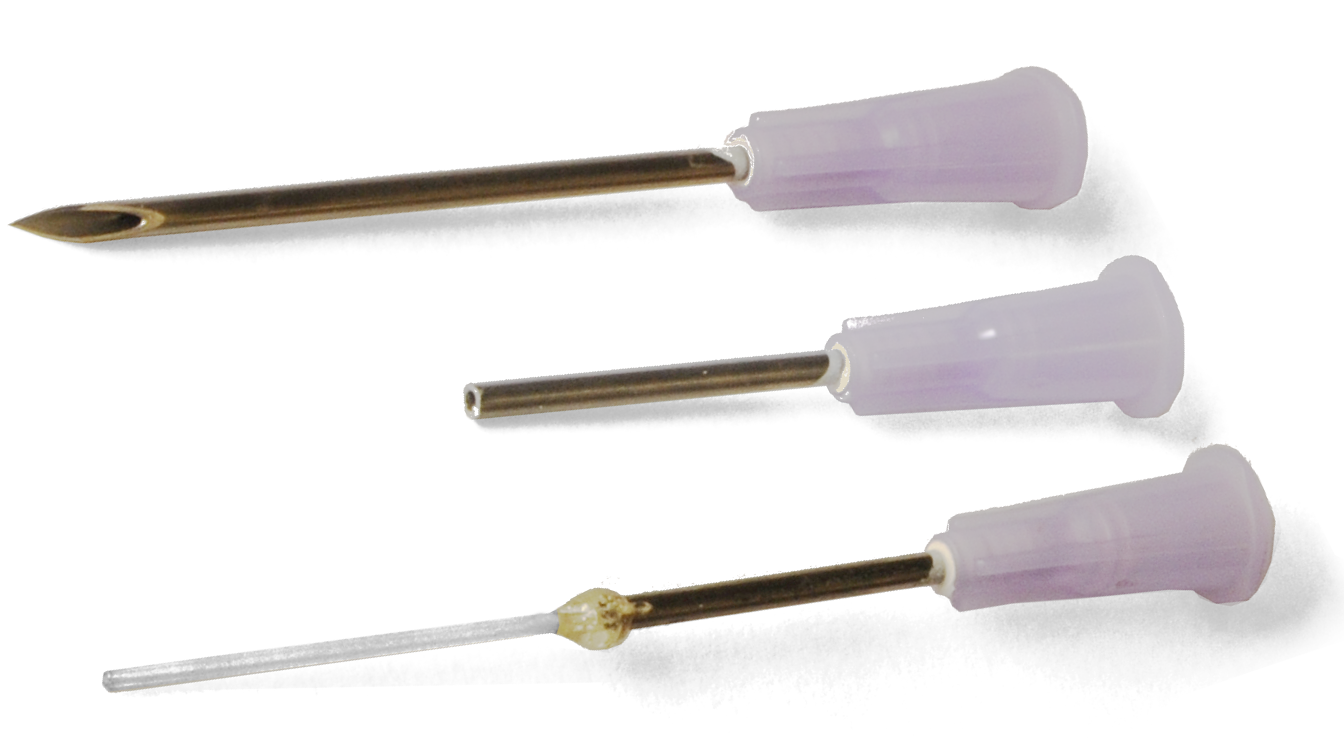
\includegraphics[width=0.4\textwidth]{papers/hdg_images/needles.png}
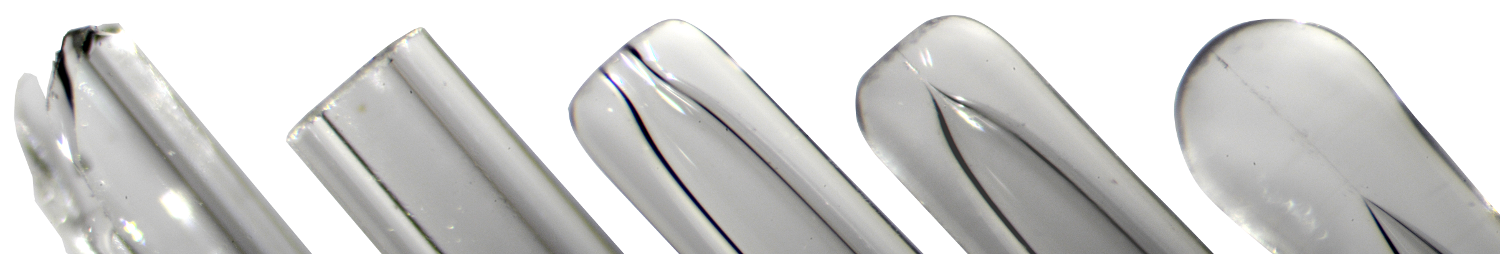
\includegraphics[width=0.35\textwidth]{papers/hdg_images/needletips.png}
\caption{Above: assembly of nozzle from
low-gauge hypodermic syringe (Luer fitting) and capillary. Below: nozzle tip
fabrication, capillary from left to right: broken, sanded, heated in a flame (I.D.
$200\,\mu$m), heated for longer (I.D. $25\,\mu$m, could be sanded down by about
$200\,\mu$m), overheated (I.D. $0\,\mu$m). \label{fig:needles}}
\end{figure}


\subsubsection{Construction}
If possible, forgo multi-platter drives, as they are more cumbersome to disassemble and have
bulky, complex actuator assemblies. The device shown in FIG. \ref{fig:photo}
is based on a single-platter drive.

\paragraph{Dismantle and cut.} After removing the hard drive cover, remove
the magnet holder, arm axis, arm, ribbon wires, circuit boards, and platters
such that only the base plate remains. Now the corner of the base plate holding
the actuator arm assembly can be cut out to yield the result shown in FIG.
\ref{fig:designschematic}. A band saw, jigsaw or powered hacksaw will be very
useful, although not necessary. The goal is to allow the tip of the arm to
protrude over the edge.

\paragraph{Expose coil leads.} Next, remove the read/write head and all
wiring leading to it, along with any connected I/O and servo circuitry. Be
careful, however, not to tear off the two strands powering the voice coil. If
they are integrated in a ribbon you wish to remove, ensure that exposed
terminals remain onto which you can solder new leads.
\begin{figure}
\centering
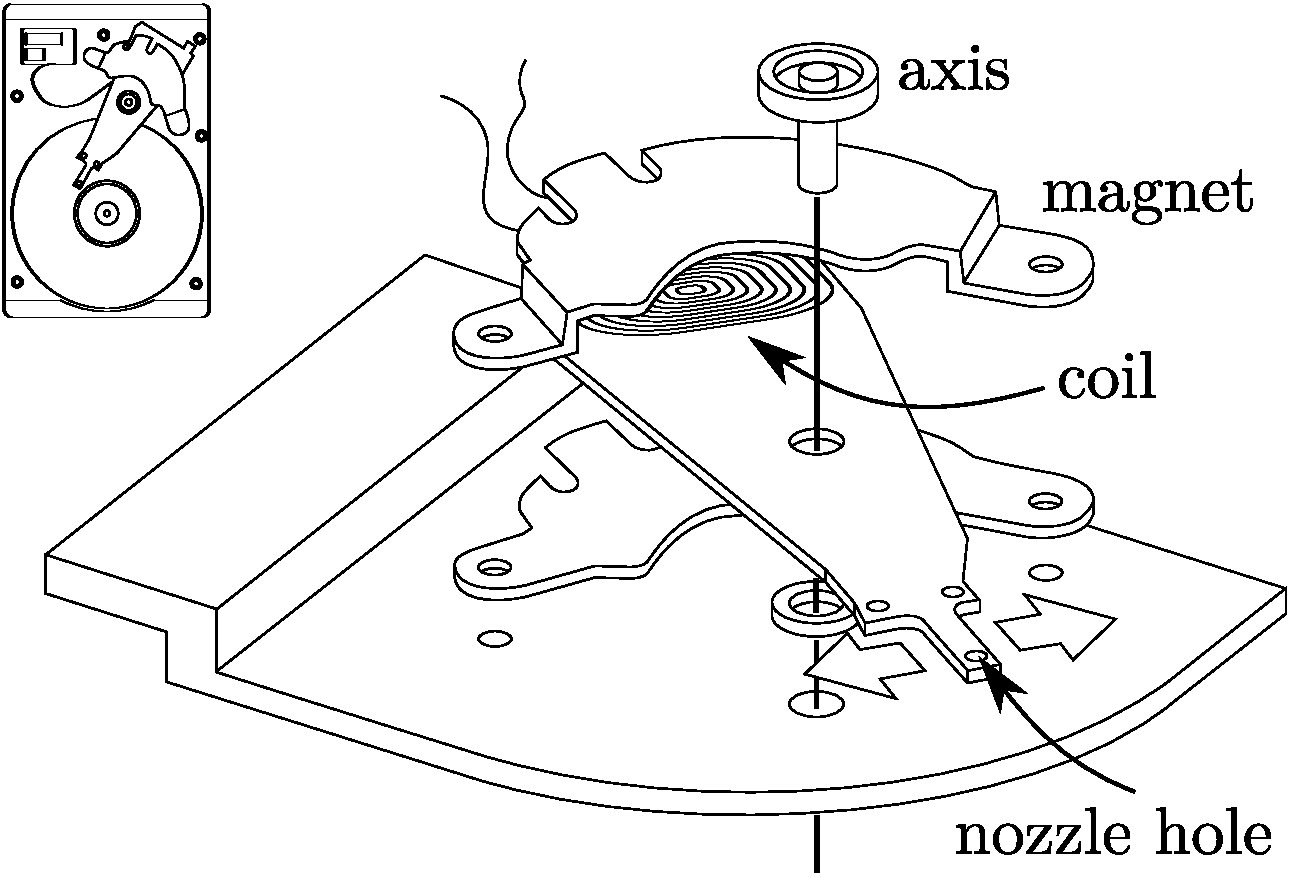
\includegraphics[width=0.4\textwidth]{papers/hdg_images/dropletgenerator_exploded.pdf}
\caption{Top view of a hard drive and exploded view of the cut-out base
plate, actuator arm, axis, and magnet assembly. \label{fig:designschematic}}
\end{figure}
\paragraph{Add protective cover.} We recommend bolting on a cover plate, such
as a small sheet of acrylic or polycarbonate, to protect the protruding arm from
accidental bending. Drill a hole through the cover to allow the nozzle to be
threaded through the arm. A severable
connection from coil to function generator is preferable to a direct wire, if
only because the voice coil leads are delicate and easily torn off. To this end, we epoxied
an audio jack into the cover and soldered the voice coil leads to it from the
bottom. 

\subsubsection{Operation}
To use the droplet generator, simply insert a nozzle through a small hole at the
tip of the actuator arm---typically at least one hole will already be present, but you may wish to drill
more---and connect the voice coil leads to the output terminal of a function
generator set to an initial peak-to-peak voltage of $1\,$V and a sinusoid frequency of
about $50\,$Hz, which should cause weak but perceptible oscillations.

\begin{figure}
\centering
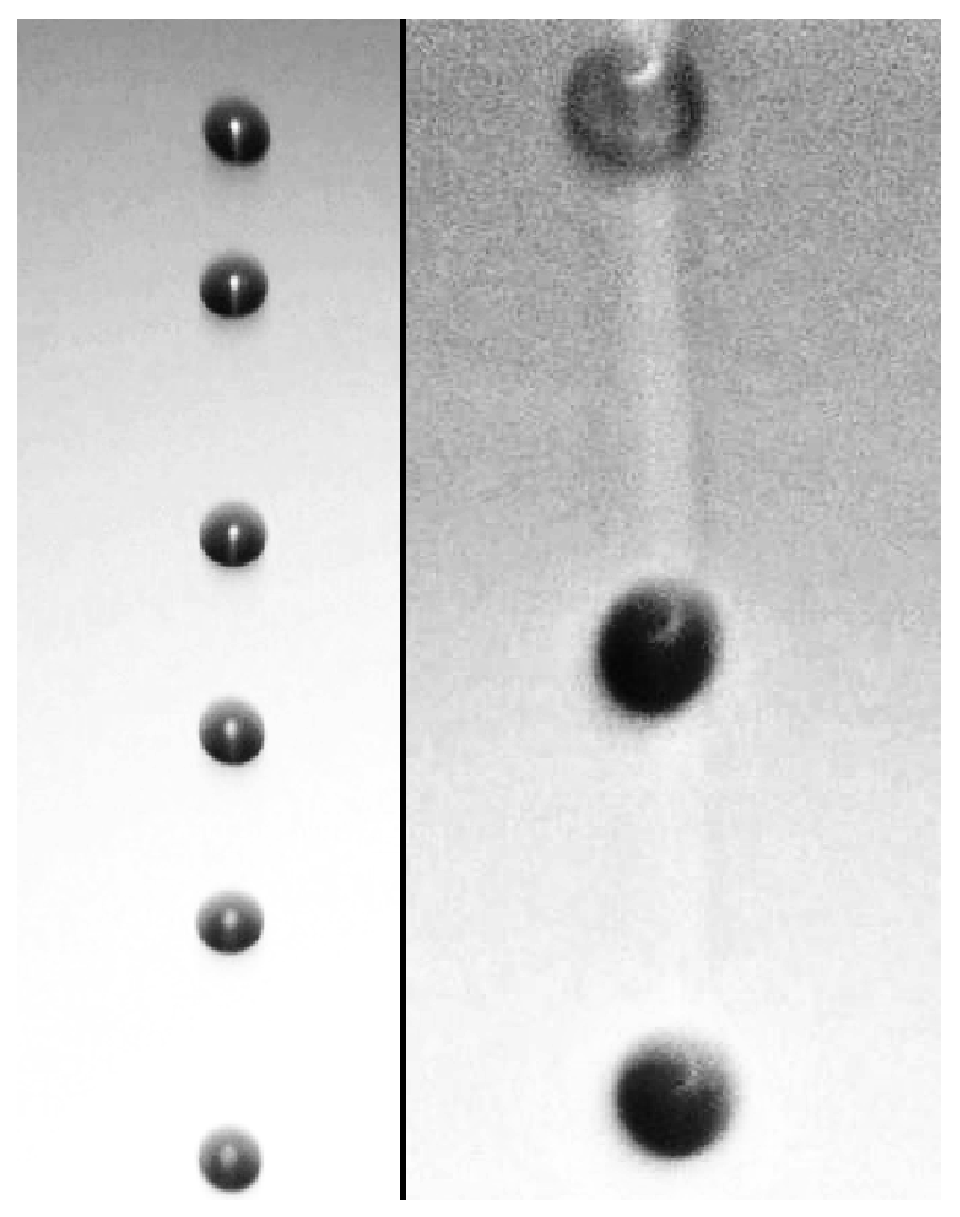
\includegraphics[width=0.3\textwidth]{papers/hdg_images/photo.eps}
\caption{Photographs of different droplet sizes ($220\,\mu$m and $386\,\mu$m,
    $f=1.990\,$kHz and $1.065\,$kHz respectively) produced with the droplet
generator shown in FIG.~\ref{fig:photo}. Scales have been cropped out. \label{fig:dropphoto}}
\end{figure}
We used existing nozzles manufactured by hand from hypodermic needle stubs and
heated glass capillaries (FIG.~\ref{fig:needles}). We make no claim that this is
the best approach to take, but we note that the interchangeability of nozzles
with Luer fittings has proved very convenient in our application. How the nozzle
can be held in place falls beyond the scope of this article; while we used an
existing setup made from machined aluminum, a small lab stand and clamp should
suffice to hold the male Luer fitting connecting the feed tube to the nozzle.

The nozzle must be supplied by an accurately calibrated syringe pump. It is
convenient to integrate a large liquid reservoir (or tap water hose) via a
T-valve between the between pump and nozzle to permit quick topping up of the
syringe. In such a setup ensure that the reservoir valve is shut closed before operation,
since pressure fluctuations at the nozzle are the most common culprit for
unstable jet breakup conditions.

As with other vibrating orifice droplet generators, it is crucial that stable
conditions are established before any experiments can begin. First, confirm that
the liquid is ejected in a single jet. Multiple jets can be due to a clogged
orifice (a mixture of distilled water and CLR®, drawn back through a
syringe, is an excellent remedy). Satellite droplets can also form secondary
jets, in which case the oscillation frequency must be adjusted or the amplitude
reduced. Satellite formation is easily detected by using a gentle air flow to
deflect the jet---if the droplets are truly monodisperse, they will all deflect
at the same angle.\cite{Strom69}


\section{Photographic verification of droplet sizes}
This is where I show pictures and tables, showing that the formula
actually works.

While there are different methods of photographing droplets, just taking
pictures in front of a strobe light has worked well.

\subsection{Colliding droplets}
\label{sec:droplet-collisions}
No droplet generation mechanism is perfect. Small fluctuations in flow rate,
unwanted harmonic vibrations and air turbulence can cause disturbances in the
stream of evenly spaced droplets -- the smaller the droplets, the more often
this happens. Occasionally, this will lead to the collision
of two droplets some distance away from the orifice.

When two drops of diameter $D_d$ collide, the diameter of the new droplet equals
\begin{equation}
    D_{d+d} = 2\sqrt[3]{2\left(\frac{D_d}{2}\right)^3} = \sqrt[3]{2} D_d \approx
    1.26 D_d.
\end{equation}

Indeed, secondary peaks will often appear in diameter histograms at precisely 126\% of
the peak diameter. As long as the underlying phenomenon is understood and kept
under control, these secondary peaks should be no cause for concern during the
calibration. Typically, photographs will confirm that a few droplets go astray
and collide with others. Since the ``real'' diameter peaks are easily discerned,
the secondary peaks can simply be ignored.

    \chapter[Interferometric Particle Imaging (IPI)]{Interferometric Particle\\ Imaging (IPI)}
    [Introductory paragraph], saying that this is also called ILIDS (invented by
    \citet{Glover95})
\section{Operating principle}
The number of fringes $N_\text{fr}$ appearing in the image has a simple linear relationship to
the droplet diametre $D_d$:
\nomenclature{$N_\text{fr}$}{Number of fringes}
\nomenclature{$\kappa$}{Scalar value relating the fringe count $N_\text{fr}$ to
the physical diameter of the particle $D_d$}
\nomenclature{$D_d$}{Physical diameter of the particle (here: droplet)}
\begin{equation}
    N_\text{fr} = \kappa D_d,
\end{equation}
where $\kappa$ is a constant derived from the optical configuration:
\begin{equation}
    \kappa = \frac{\arcsin\left(\frac{D_a}{2z}\right)}{\lambda}
    \left(\cos\frac{\phi}{2} - \frac{m \sin\frac{\phi}{2}}{\sqrt{m^2 + 1 -
    2m\cos \frac{\phi}{2}}}\right).
    \label{kappa}
\end{equation}

In the above expression $D_a$ is the aperture diametre, $z$ is the distance of
the lens to the laser sheet, $\phi$ is the off-axis angle (90 degrees in most
setups, including ours), and $m$ is the relative refractive index of the
droplets (1.333 for water in air).

As a consequence of geometrical optics, the distance $s_x$ (in pixels) between two
adjacent fringes has a linear relationship with the defocussing distance $\Delta
z$, where $M$ is the magnification, $d_{p,x}$ is the physical size of a
camera sensor pixel, and $\Delta \theta$ is the angle subtended by two adjacent
fringes entering the lens \cite{Pan06}:
\nomenclature{$\Delta \theta$}{Angular spacing between two adjacent fringes}
\nomenclature{$\Delta z$}{Distance along the $z$-axis between the focal plane of
the lens and the light sheet}
\nomenclature{$M$}{Magnification}
\nomenclature{$s_x$}{Distance, in pixels, between two adjacent fringes}
\nomenclature{$d_{p,x}; d_{p,y}$}{Physical dimensions of a pixel on the camera's
CCD sensor}
\begin{equation}
  s_x = \frac{\Delta \theta \Delta z}{M d_{p,x}} 
  \label{fringedistance-pixels}
\end{equation}
Of course, equation \eqref{fringedistance-pixels} is only meaningful where $\Delta z \gg
0$. If the image is (approximately) focussed, fringes will give way to a sharp
image of either both glare points or a single bright spot -- depending on
diffraction effects and the camera's resolution.

(Fill in more details here.)
\subsection{Influence of the scattering angle $\phi$}
The scattering angle $\phi$ determines the relative contribution of 
different scattering orders of light to the imaged fringe pattern. Both
geometric optics \cite{Vandehulst12} and Mie theory provide methods to compute
the total scattered intensity for a given $\phi$ and $m$. Some examples can be
found in \citet{Kawaguchi02} and \citet{Mounaim99}. The geometric analysis
approach is not valid beyond $\phi > 70^\circ$, as the first-order
scattered beam ($p=1$) is not visible from this angle \cite{Glover95}.

While authors have identified several forward angles as optimal for their
applications, e.g. $\phi = 45^\circ$ \cite{Glover95} or $\phi = 66^\circ$
\cite{Mounaim99}, such configurations inevitably result in a variation in $z$,
leading to different degrees of defocussing across the image -- unless the
camera itself is angled with respect to the lens to correct for this
aberration (the so-called \emph{Scheimpflug condition}). Since the latter
approach requires specialized optical equipment, $\phi = 90^\circ$ is used in
many setups, including the one in this paper (Section \ref{sec:ipi-setup}).

\subsection{Optical limits on fringe detection}
\label{sec:ipi-fringelimits}
Optics impose theoretical and practical size limits on the droplets to be
measured. We will outline them in the following paragraphs; the reader is
referred to \citet{Damaschke02} for a more detailed analysis.

\paragraph{Nyquist criterion for the fringe density.}
The Nyquist criterion requires that for the camera to be able to resolve a pair
of neighbouring fringes, they must be at least two pixels apart. This can easily
be achieved by sufficiently defocussing the lens, which widens the fringe image,
increasing the number of pixels covered by each fringe. The lens mechanics
permitting, any arbitrarily large droplet can thus be measured after a quick
adjustment. In theory, this correction is effective until the defocussed droplet
image is too large for the CCD sensor, and fringes are cut off. In practice,
overlap and noise (see below) will cause significant problems long before the
image can be defocussed beyond the sensor edges.

\paragraph{Overlapping droplet images.}
As the lens is brought farther out of focus, the droplet images dilate and
overlap one another. Increasing levels of overlap frustrate attempts to identify
and analyse the images. Although the slit aperture method discussed in Chapter
\ref{chp:slit-aperture} was developed to circumvent this effect, it is not
entirely immune to it -- particularly when droplets are very closely spaced, as
they often are when vibrating orifice droplet generators are used. See Section
\ref{sec:ipi-overlap} for a more in-depth discussion.

\paragraph{Signal-to-noise ratio.}
Image noise is a significant source of trouble in IPI analysis -- indeed, many
droplet images must be discarded as data sources because they are too noisy.
Noise affects small droplets in particular because they scatter less light than
larger ones,\footnote{The scattered intensity grows with the cross-section of
the droplet} but it is also a problem with deeply out-of-focus images of very
large droplets, as dilated droplet images spread the same amount of light over a
greater area on the camera sensor. As a result, they are darker on average than
less defocussed images. 

\paragraph{Minimum droplet size.}
\citet{Damaschke02} argue that the smallest measurable droplet is one that
produces exactly one fringe covered by the aperture. We propose that, at least
in theory, a partial fringe should be measurable if its image is sufficiently
zero-padded before the Fourier transform is applied to it. \emph{This might need
elaboration.} In practice, the intensity of scattered light is likely to drop
below an acceptable level before the fringes become too large, and noise (see
above) will become the overwhelming problem. The researcher should also be aware
that the assumptions of geometric optics that underlie \eqref{kappa} do
not hold for small droplets (see Section \ref{sec:mie-error} for details).

\section{Setup}
\label{sec:ipi-setup}
(How it's set up, what cameras, what lenses, what laser, timer box, software,
etc.)

\section{Common problems and sources of error}
\subsection{Too much overlap}
\label{sec:ipi-overlap}
This is a section where I refer to the paper that calculates overlap
probabilities/overlap coefficients. I explain that many droplets are mis-identified (either high-freq
is seen as low-freq, or noise is seen as high-freq) and where I point out that
while Hanning windows and min-distance/max-overlap filters help a little bit,
they also skew the representativeness of the sample because only small,
dispersed satellites are outside of the main flow.

I explain that there isn't really an easy method of fixing this, and that any
time spent attempting to deal with the problem is better spent building a slit
aperture system, as described in the next chapter.

\subsection{Thin lens assumption}
What matters is the Numerical Aperture (NA), which is (the sine of half of) the
collection angle. When we have a simple lens, we can calculate this as
\begin{equation}
    \mathrm{NA} = \sin \frac{d_a}{2z}\\
    3\alpha \rho = \sqrt{2 \lambda x r}
\end{equation}

The Dantec manual suggests using the distance from light sheet to front of the
lens for $z$, and the ratio of min focal length and max f-number to find $d_a$.
This, however, does not result in an accurate value for the collection angle
with all lenses.

We are assuming, then, that the effective aperture (the entrance pupil) always
stays constant throughout the focussing range of the lens. This is not
necessarily the case, as there are lenses which change both the physical and the
virtual size of the aperture when focussing. The best way to get the collecting
angle is to go by magnification

Here is where I make the claim that it is impossible to determine the actual
exact value for the numerical aperture of the lens. Similarly, it can be quite
difficult to determine the accurate distance from light sheet to lens aperture
(even though the latter measurement is more forgiving, since the distances are
far greater).

\subsection{Error in the Mie approximation at small sizes}
\label{sec:mie-error}
As outlined in paper ... geometric optics deviate from the true Mie scattering
field when sizes are very small.

\subsection{Centre discrepancies}
The most challenging stage of the measurement process is the detection of the
defocussed droplet images. Since the defocussed images assume the shape of the
aperture, which is wide open in most applications,\footnote{see Chapter
\ref{chapter:slitaperture} for a discussion of the benefits of non-circular
apertures.} they are typically circular. Moreover, they are all more or less of
the same size as a consequence of equation \eqref{}.

\begin{figure}
\centering
%\includegraphics[]{droplet-overlap.jpg}
\caption{Overlapping defocussed droplet images}
\label{fig:droplet-overlap}
\end{figure}

\section{Eliminating centre discrepancies and the need for camera calibration}
%TODO: Say that the bulk of the following work is from Kosch and Ashgriz,
%submitted to journal/conference XYZ
It thus stands to reason that a simple circle detection technique would suffice
to detect the droplet images in the photos. A polar adaptation of the Hough
accumulator technique (such as the OpenCV implementation
\texttt{cv2.HoughCircles()}) or a correlation-based pattern matching method
(e.g. \texttt{cv2.matchTemplate()}) are both obvious choices for this task.  The
problem of \emph{droplet overlap}, however, can thwart such efforts (Figure
\ref{fig:droplet-overlap}). This happens particularly when large droplets are to
be measured, because their many fringes require larger defocussed images to
resolve clearly. Indeed, in regions of high droplet density, it can be impossible
to reliably detect the circular fringe images using the methods mentioned above.

Nevertheless, once droplet image positions are established with confidence, overlap can be
dealt with to a degree: known overlapping regions can either be excluded
entirely or serve to help find maximum-likelihood frequency peaks for their
respective tributary droplet images.

Since the detection of droplet images is so essential, the Dantec DynamicStudio
software extracts the droplets' positions from the focussed photo, and then maps
those positions onto the defocussed photo based on a set of camera calibration
photos. This method is sound in principle, but often yields unsatisfactory
mappings in practice, likely whenever the calibration target plate (Figure
\ref{fig:dottarget}) is not precisely aligned with the laser sheet. In Section
\ref{sec:calibration-improvement}, we describe a more accurate and robust method
of finding the mapping based directly on the pair of droplet photos. 

Since the mapping error is often a perspectivity, the simple manual
$x/y$-shift that can be applied in the DynamicStudio software after calibration
is not a sufficient adjustment.

Dantec supplies a \emph{standard dot target}, a white $10 \times 10\,
\mathrm{cm}^2$ plate engraved with a pattern of black dots (Figure
\ref{fig:dottarget}). The plate is to be mounted such that its surface coincides
perfectly with the laser sheet. Both cameras are then focussed on the dot
pattern, and a photo is taken with both. This allows the DynamicStudio software
to calculate the transformation matrix between target plate and
image for each camera:
\begin{equation}
\left[\begin{array}{c} x'\\ y'\\ z'\\ r' \end{array} \right]
=
\left[ \begin{array}{cccc}
S_x & A_{yx} & A_{zx} & T_x \\
A_{xy} & S_y & A_{zy} & T_y \\
A_{xz} & A_{xy} & S_z & T_z \\
P_x & P_y & P_z & S_0
\end{array} \right]
\left[ \begin{array}{c} x\\ y \\ z \\ 1 \end{array} \right].
\end{equation}

In practice, $P_{x,y,z} = 0$ and $S_z = S_0 = 1$, such that the mapping is
affine (although we will later show that this need not be the case). The
$z$-components (third row/column) are ignored, such that a $3 \times 3$ matrix
suffices for the purposes of this discussion:
\begin{equation}
\left[\begin{array}{c} x'\\ y'\\ r' \end{array} \right]
=
\left[ \begin{array}{ccc}
S_x & A_{yx} &  T_x \\
A_{xy} & S_y &  T_y \\
P_x & P_y & S_0
\end{array} \right]
\left[ \begin{array}{c} x\\ y \\ 1 \end{array} \right].
\end{equation}

The DynamicStudio software thus finds the camera matrices
$\mathbf{P}_\text{foc}$ and $\mathbf{P}_\text{def}$ mapping the
object (the target plate) onto the two camera images:\footnote{Henceforth, the
    subscripts ``foc'' and ``def'' shall designate the focussed and defocussed
    cameras, respectively -- even though both are focussed when the initial
calibration photo is taken.}
\begin{align}
    \mathbf{x}_\text{foc}' &= \mathbf{P}_\text{foc} \, \mathbf{x} \\
    \mathbf{x}_\text{def}' &= \mathbf{P}_\text{def} \, \mathbf{x}.
\end{align}

It follows that the quotient of the two matrices, also known as the homography
\begin{equation}
    \mathbf{H} = \mathbf{P}_\text{def} \, \mathbf{P}_\text{foc}
\end{equation}
can be used to map the focussed image onto the defocussed image:
\begin{equation}
    \mathbf{H}\, \mathbf{x}_\text{foc}' = \mathbf{x}_\text{def}'.
    \label{homography-definition}
\end{equation}

In practice, it is not always possible to ensure that the dot target plate is
aligned with the laser light sheet to absolute perfection. This introduces a
perspective error in the homography matrix $\mathbf{H}$. Figure
\ref{fig:plate-calibration} shows that even though the calibration images
are mapped perfectly, there is a perspective error in Figure
\ref{fig:drop-calibration-off}.

\begin{figure}
        \centering
        \begin{subfigure}[b]{0.45\textheight}
                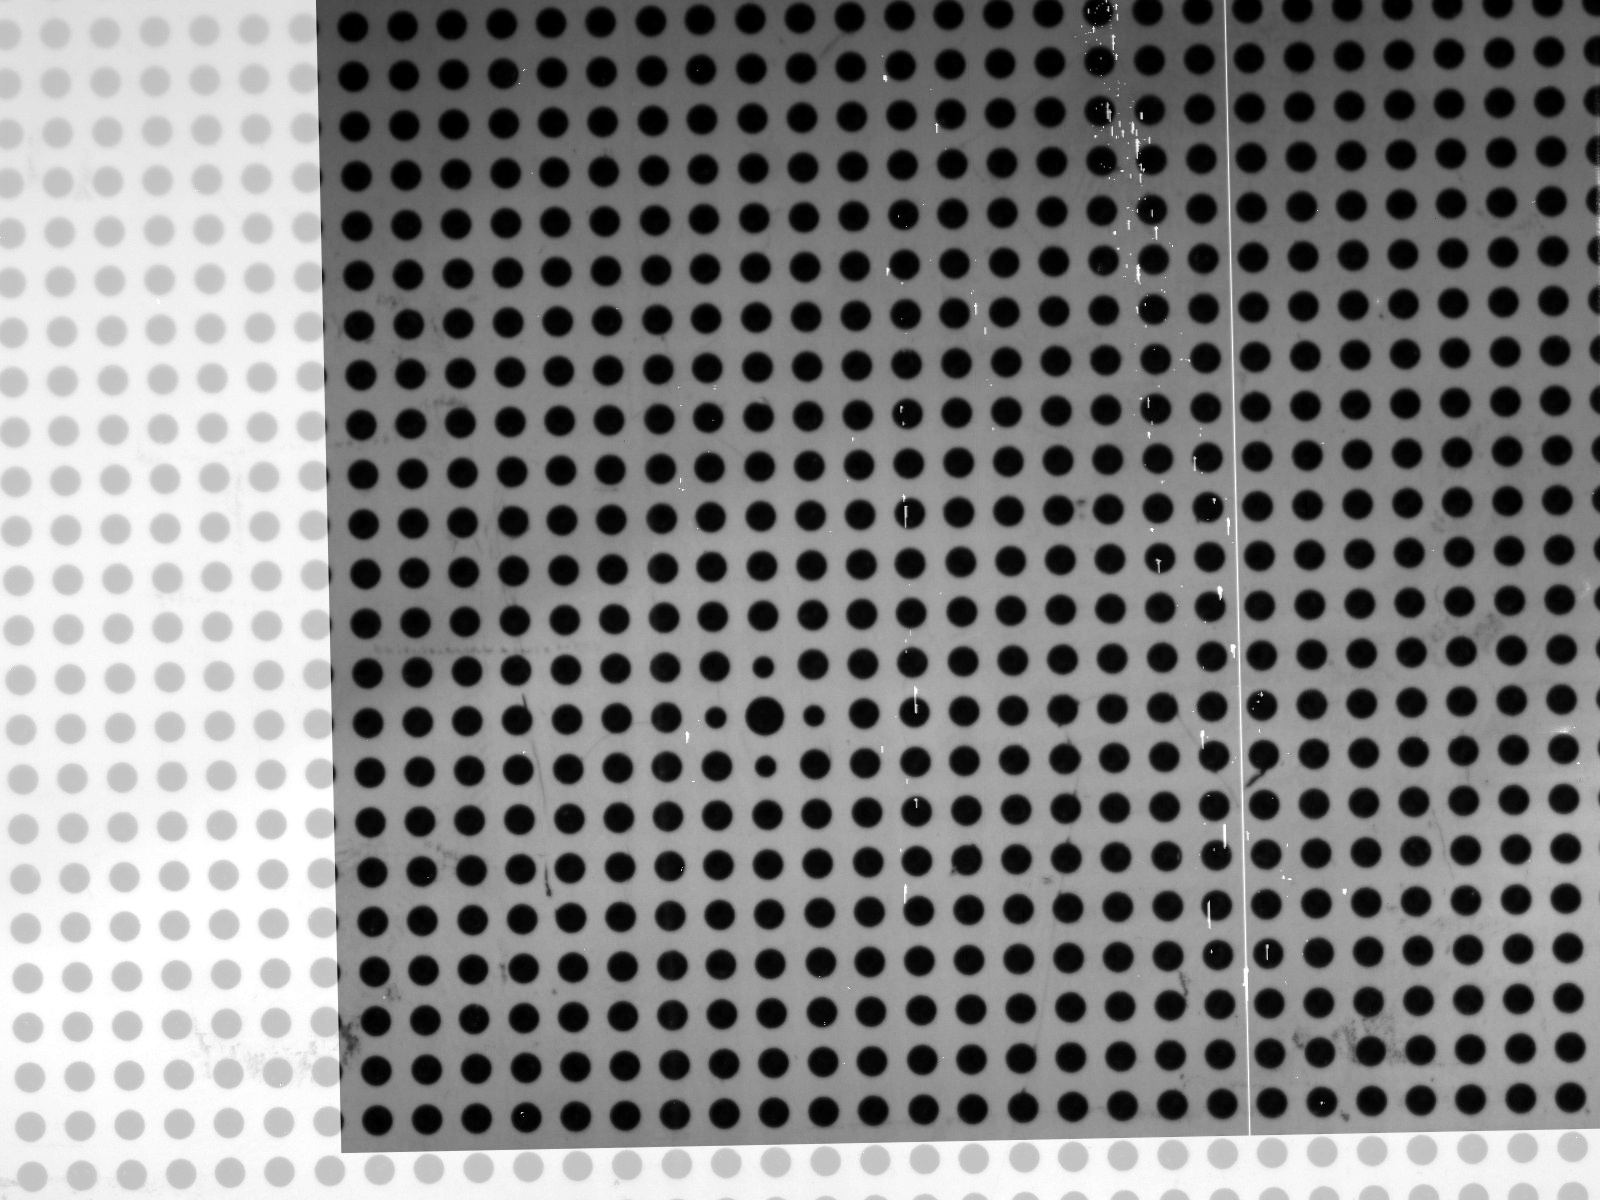
\includegraphics[height=0.4\textheight]{img/plate-calibration.jpg}
                \caption{Focussed camera image, after applying homography, is
                    superimposed onto defocussed camera image of dot target
                plate.}
                \label{fig:plate-calibration}
        \end{subfigure}
        \vskip 2.5em
        \begin{subfigure}[b]{0.45\textheight}
            \centering
                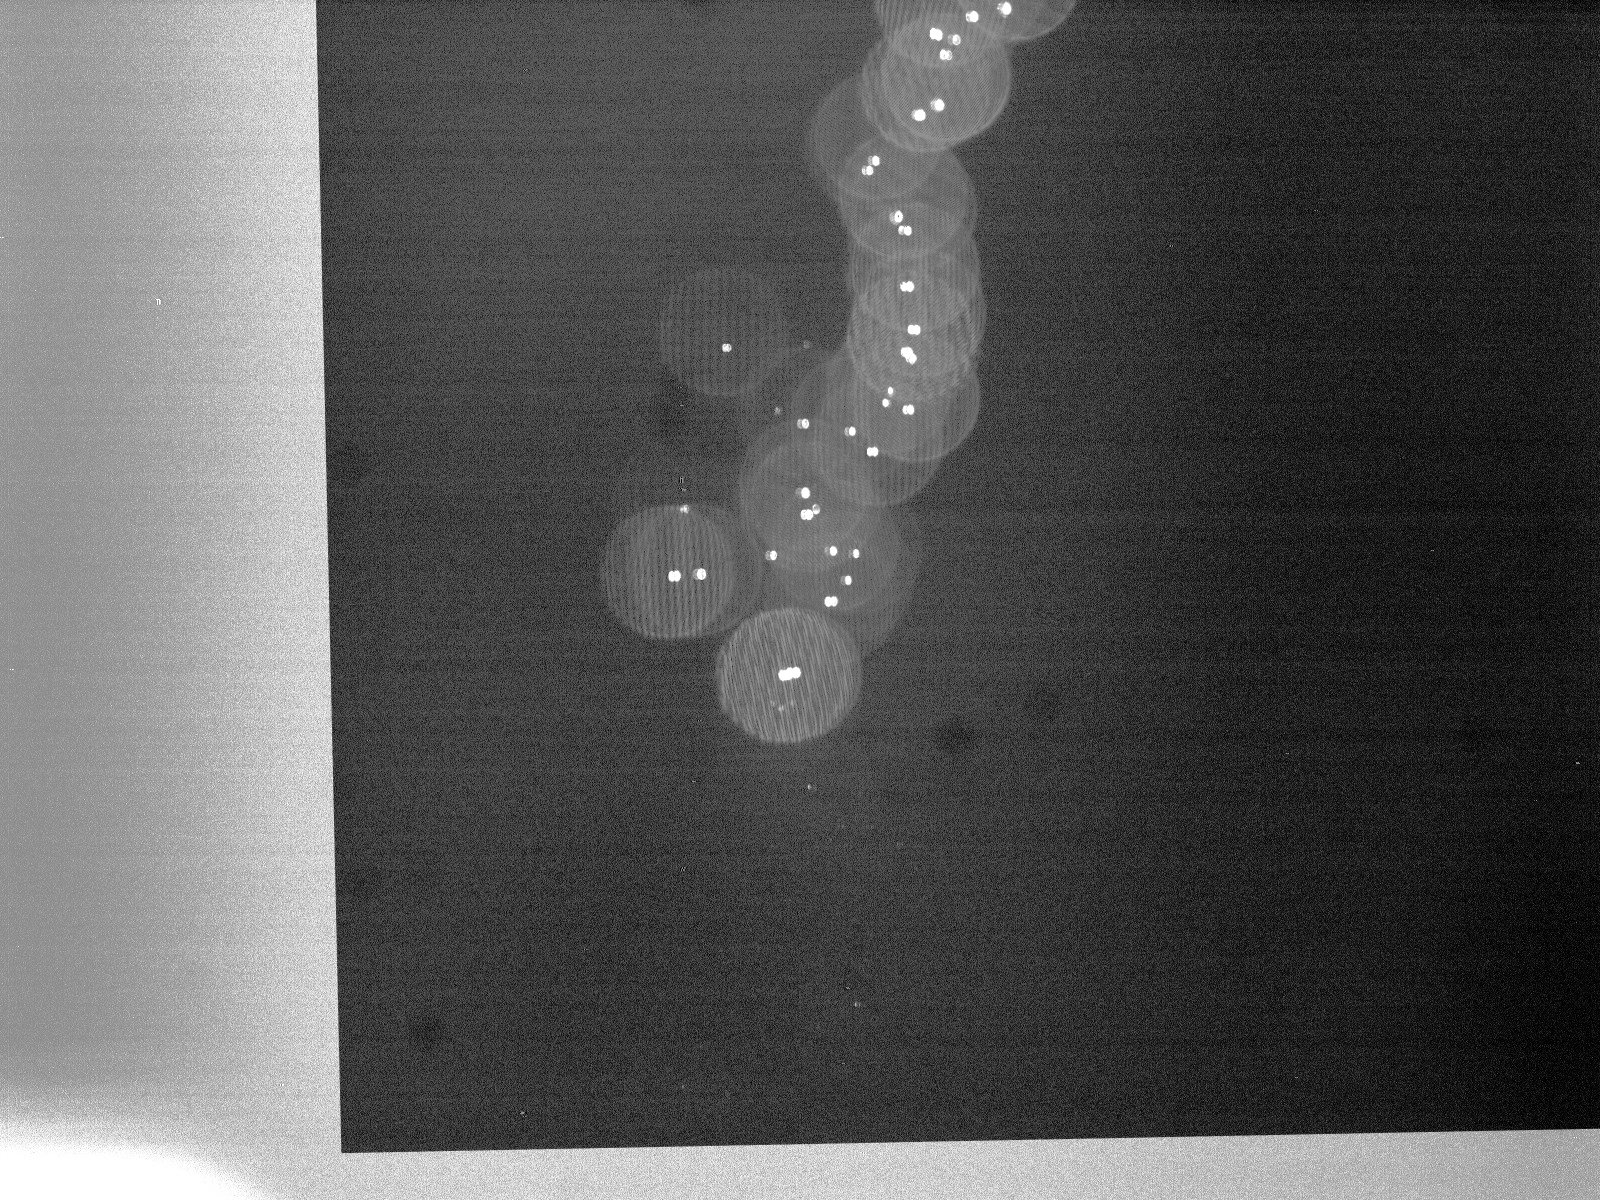
\includegraphics[height=0.4\textheight]{img/drop-calibration-off.jpg}
                \caption{Focussed camera image, after applying homography
                    derived from the calibration images, is superimposed onto
                defocussed camera image of droplets.}
                \label{fig:drop-calibration-off}
        \end{subfigure}
        \caption{Illustration of the perspective error from misaligned
        calibration target plate}
        \label{fig:calibration-error}
\end{figure}

To correct for this error, we can use image registration techniques to derive
the homography mapping \emph{directly} from the focussed and defocussed droplet
images, doing away with the need for calibration pictures altogether. Once we
find the corrected homography $\mathbf{\Hhat}$, we use it to find
\begin{equation}
    \mathbf{\Phat}_\text{def} = \mathbf{\Hhat} \, \mathbf{P}_\text{foc},
    \label{corrected-homography-use}
\end{equation}
which can be manually entered into the DynamicStudio software to replace
$\mathbf{P}_\text{def}$.

\subsubsection{Finding the corrected homography}
Image registration is the process of finding the best possible mapping of one
image onto another -- in other words, it is a term for homography-finding
techniques. The basic process comprises three steps:
\begin{enumerate}
    \item \textbf{Feature detection:} Finding ``features'', i.e. unique points or regions in the images --
        such as corners, arcs, or contrasting regions which stay
        relatively stable even when the image is thresholded.
    \item \textbf{Feature description:} Converting the detected features into
        numerical vectors.
    \item \textbf{Feature matching:} Finding good correspondences between
        features in the two images -- this often requires inlier/outlier
        decision-making, e.g. RANSAC.
\end{enumerate}

Naturally, image registration is impossible to achieve between our focussed and
defocussed images. We therefore first apply the following steps to our focussed
image:

\begin{enumerate}
    \item Mask the image, excluding all areas that are known not to contain
        droplets.
    \item Subtract the pixel-wise minimum or mean taken over all images taken by
        the camera. This step will remove hot pixels on the camera's CCD sensor
        and other static noise.
    \item Erode the image, using a $3 \times 3$ or $5 \times 5$ kernel. This
        will close any remaining bright pixels which are likely noise.
    \item Locate the intensity peaks in the remaining image.
    \item Fill a new image with black, then draw white circles of diameter $D_d$
        onto it, centered at the respective positions of the intensity peaks
        detected in the focussed image.
\end{enumerate}

The result of these operations is shown in Figure \ref{fig:dilating-droplet-dots}.
\begin{figure}
        \centering
        \begin{subfigure}[b]{0.45\textheight}
                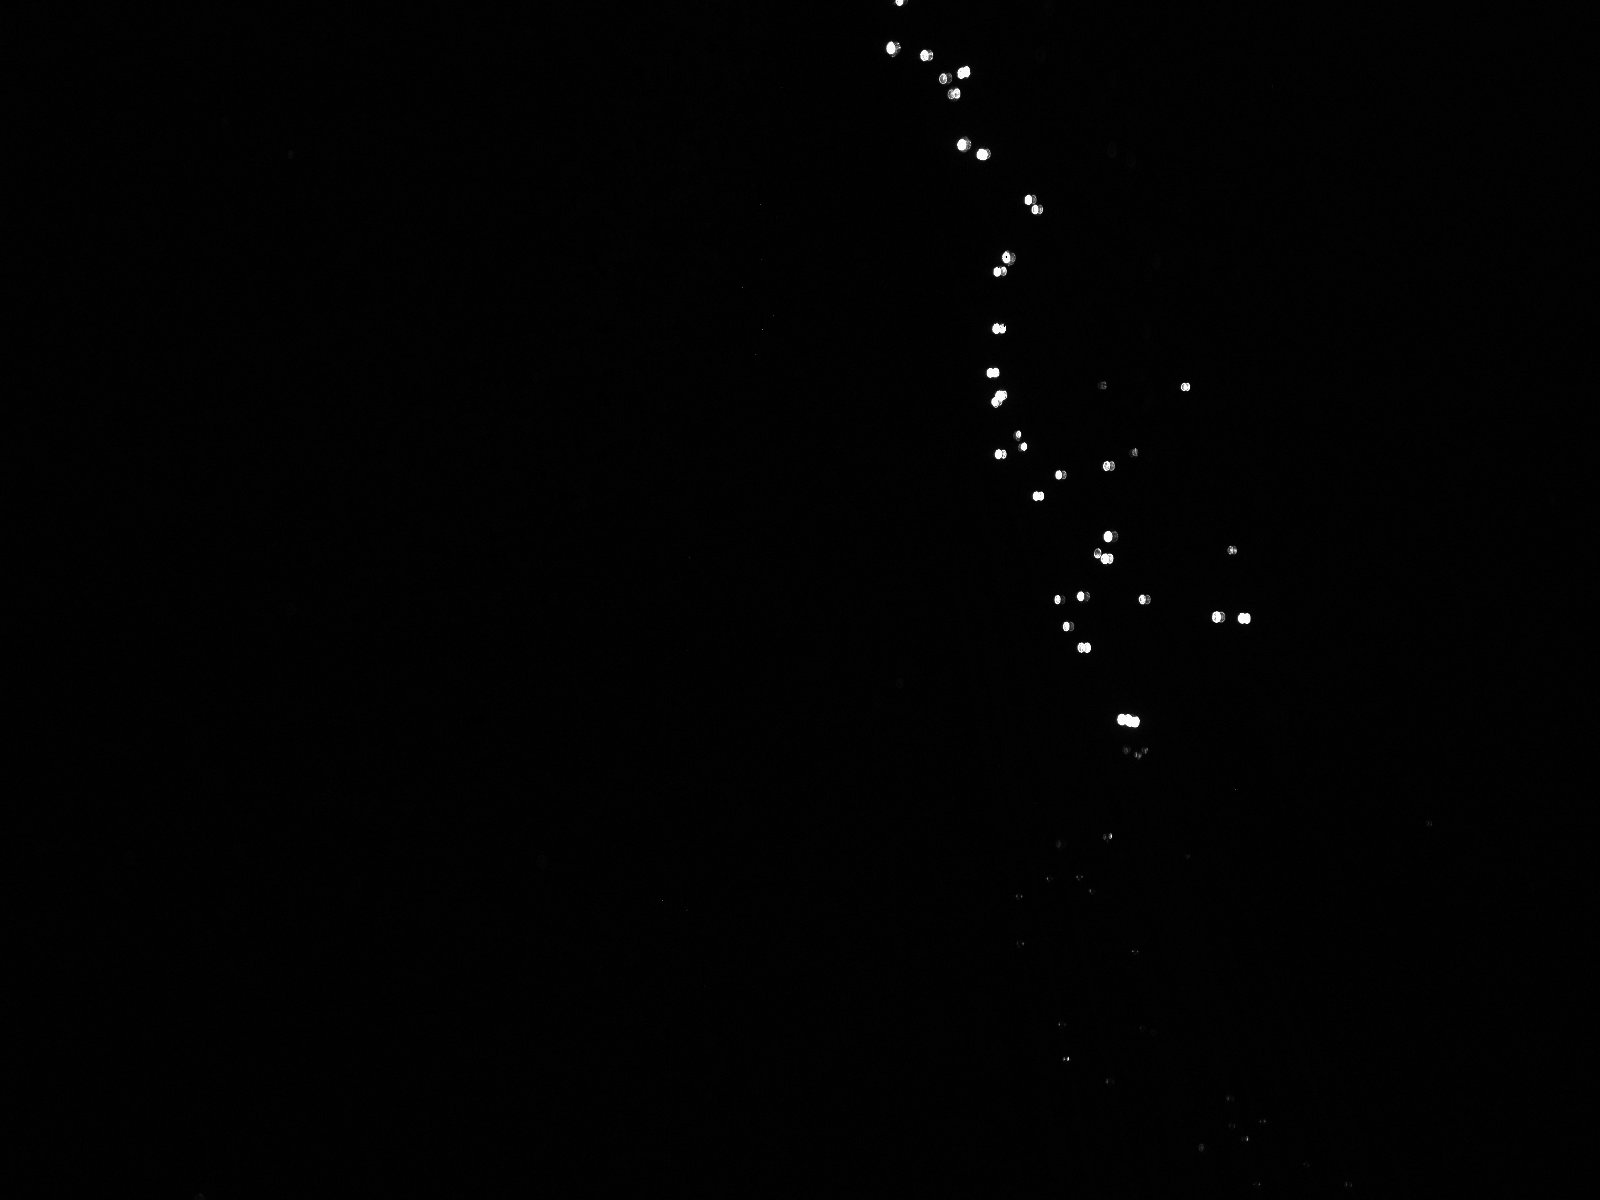
\includegraphics[height=0.4\textheight]{img/focussed.jpg}
                \caption{Focussed camera image.}
                \label{fig:focussed}
        \end{subfigure}
        \vskip 2.5em
        \begin{subfigure}[b]{0.45\textheight}
            \centering
                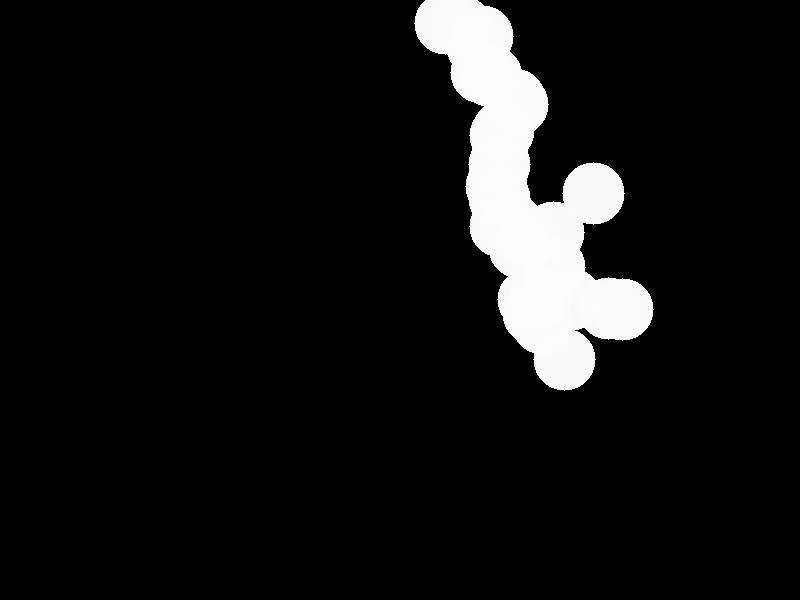
\includegraphics[height=0.4\textheight]{img/focussed-dilated.jpg}
                \caption{Simulated defocussed camera image based on focussed
                camera image, used for registration.}
                \label{fig:focussed-dilated}
        \end{subfigure}
        \caption{Using the focussed image to simulate the defocussed image for
        registration}
        \label{fig:dilating-droplet-dots}
\end{figure}

Image registration algorithms are often not very robust. This is especially true
when the two pictures are not photos taken from slightly different angles.
Moreover, image processing algorithms have runtime complexities that grow at
least with the area of the image. We therefore prepare our focussed image by
shrinking it to half the size (transformation $\mathbf{S}_{0.5}$) and mirroring
it horizontally (transformation $\mathbf{M}_h$).

Our image registration algorithm makes use of the affine invariance of the
\textsc{asift}
algorithm \cite{}, but instead of the patented \textsc{sift} detector/descriptor pair
\cite{}, we use \textsc{orb} \cite{} for feature detection and \textsc{brief} \cite{} for feature
description. A more detailed explanation of the algorithm can be found in
Appendix \ref{appendix:asift}. Figure \ref{fig:asift-matching} shows a
successful mapping between focussed and defocussed images.

The homography found by the registration algorithm, $\mathbf{K}$, must now be
converted into a homography between the original images, $\mathbf{\Hhat}$. We
see that
\begin{equation}
    \mathbf{K}\, \mathbf{M}_h\, \mathbf{S}_{0.5}\, \mathbf{P}_\text{foc} =
    \mathbf{S}_{0.5} \mathbf{P}_\text{def};
\end{equation}
note here that the mirroring operation is applied only on one side of the
equation, since the original images are mirrored and the goal is to undo this
before running the image registration. To bring this into the form required by
\eqref{homography-definition}, we write
\begin{align}
    \mathbf{S}_{0.5}^{-1}\, \mathbf{K}\, \mathbf{M}_h\, \mathbf{S}_{0.5}\,
    \mathbf{P}_\text{foc} &=
     \mathbf{S}_{0.5}^{-1}\, \mathbf{S}_{0.5} \mathbf{P}_\text{def} \\
     &= \mathbf{P}_\text{def}
 \end{align}
Finally, it turns out that DynamicStudio violates convention by placing the
coordinate origin at the bottom left corner of the image. We must therefore 
pre- and post-multiply by $\mathbf{M}_v^{\pm 1}$ to arrive at our final
expression for $\mathbf{\Hhat}$:
\begin{equation}
    \mathbf{\Hhat} = \mathbf{M}_v\, \mathbf{S}_{0.5}^{-1}\, \mathbf{K}\,
    \mathbf{M}_h\, \mathbf{S}_{0.5}\, \mathbf{M}_v^{-1}.
\end{equation}
We shall provide the transformation matrices for convenience:
\begin{align}
    \mathbf{M}_h &= \left[ \begin{array}{ccc}
    -1 & 0 & \text{(image width)} \\
            0 & 1 & 0 \\
            0 & 0 & 1
    \end{array} \right] \\
    \mathbf{M}_v &= \left[ \begin{array}{ccc}
            1 & 0 & 0 \\
    0 & -1 & \text{(image height)} \\
            0 & 0 & 1
    \end{array} \right] \\
    \mathbf{S}_{0.5} &= \left[ \begin{array}{ccc}
            0.5 & 0 & 0 \\
    0 & 0.5 & 0 \\
            0 & 0 & 1
    \end{array} \right]
\end{align}
  
The improved matching achieved using $\mathbf{\Phat}_\text{def}$ is shown in
Figure \ref{fig:drop-calibration-corrected}. Having calculated $\mathbf{\Phat}_\text{def}$ using
equation \eqref{corrected-homography-use}, we can import it into DynamicStudio
to improve the identification of droplets.

\begin{figure}[t]
    \centering
    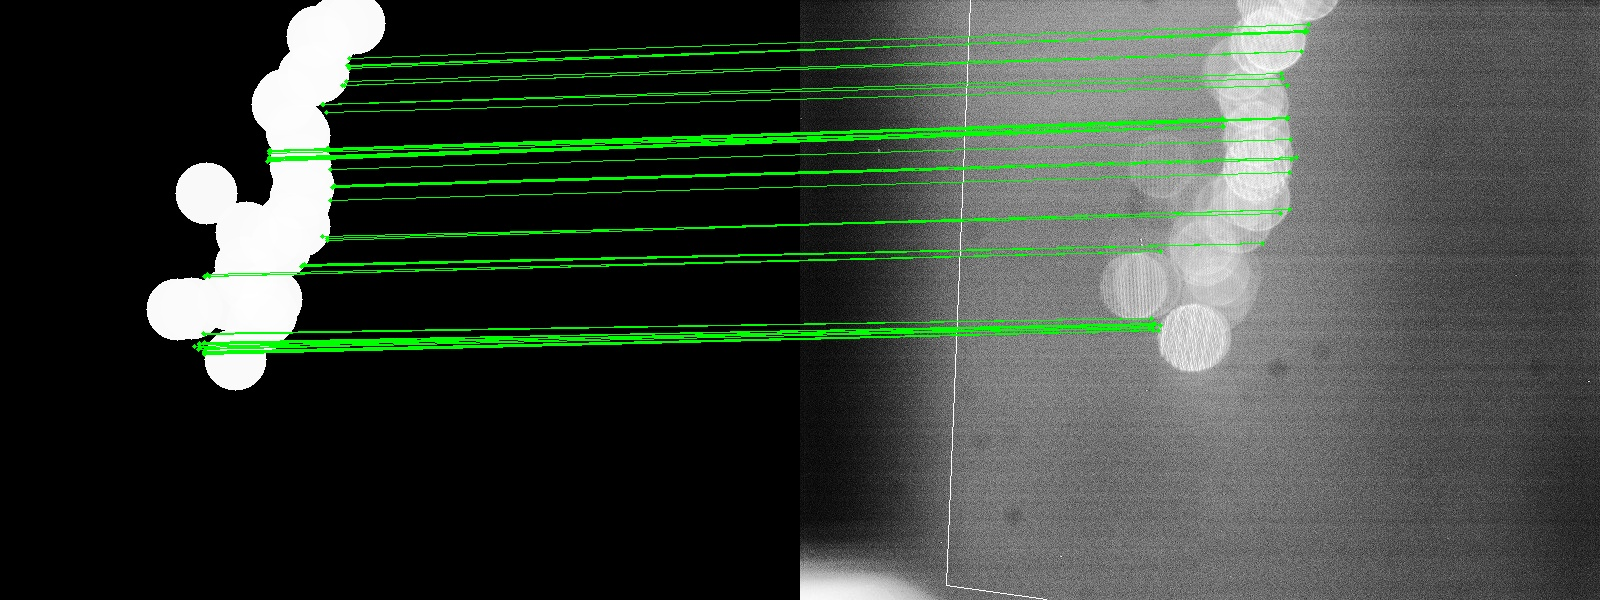
\includegraphics[width=\textwidth]{img/asift-matching.jpg}
    \caption{Matching between focussed and defocussed images.}
    \label{fig:asift-matching}
\end{figure}

\begin{figure}[t]
    \centering
    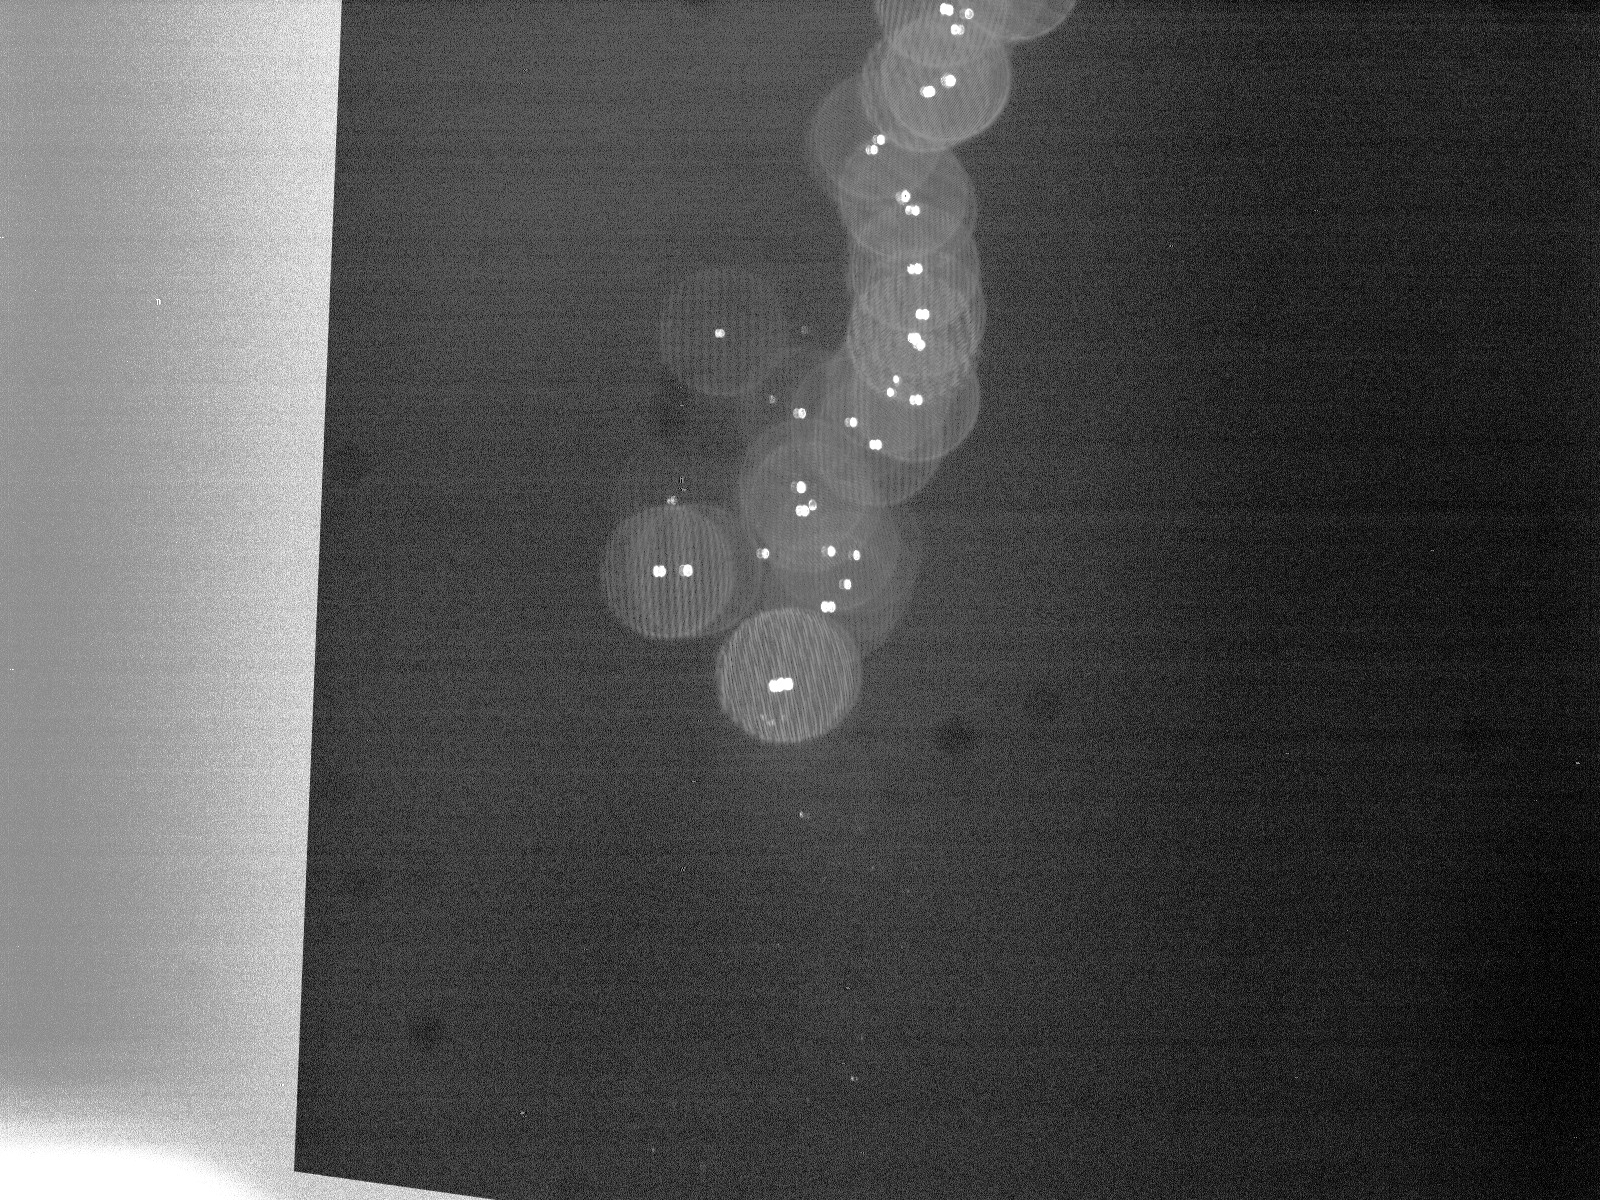
\includegraphics[width=0.45\textheight]{img/drop-calibration-corrected.jpg}
    \caption{Focussed camera image, after applying homography
        derived from image registration, is superimposed onto defocussed
    camera image of droplets.}
    \label{fig:drop-calibration-corrected}
\end{figure}

%%%%%%%%%%%%%%%%%%%%%%%%%%%%%%%%%%%%%%%%%%%%%%%%%%%%%%%%%%%%%%%%%%%%%%%%%%%
%%%%%%%%%%%%%%%%%%%%%%%%%%%%%%%%%%%%%%%%%%%%%%%%%%%%%%%%%%%%%%%%%%%%%%%%%%%

%%%%%%%%%%%%%%%%%%%%%%%%%%%%%%%%%%%%%%%%%%%%%%%%%%%%%%%%%%%%%%%%%%%%%%%%%%%%%%%
%%%%%%%%%%%%%%%%%%%%%%%%%%%%%%%%%%%%%%%%%%%%%%%%%%%%%%%%%%%%%%%%%%%%%%%%%%%%%%%
%                            SLIT APERTURES                                   %
%%%%%%%%%%%%%%%%%%%%%%%%%%%%%%%%%%%%%%%%%%%%%%%%%%%%%%%%%%%%%%%%%%%%%%%%%%%%%%%
%%%%%%%%%%%%%%%%%%%%%%%%%%%%%%%%%%%%%%%%%%%%%%%%%%%%%%%%%%%%%%%%%%%%%%%%%%%%%%%

\chapter[Particle sizing with a slit aperture]{Particle sizing with \\a slit aperture}
\label{chp:slit-aperture}
As we discussed in Section \ref{sec:ipi-overlap}, many otherwise well-executed IPI
measurements are thwarted by overlapping defocussed droplet images.
This problem is never more apparent than in efforts to calibrate
the system using a vibrating orifice droplet generator, as the droplets produced
thereby are spaced very closely and produce heavily overlapping defocussed
images. Fortunately, there exists a simple and reliable technique to deal with
this problem: a slit aperture, installed directly in front of the lens, masks
the defocussed droplet images such that only a thin strip across their center
passes through the lens. The effect is shown in Figure \ref{fig:globalsizing}. 

The idea of optically compressing an image in one direction is
well-known from the field of spectroscopy. It was first introduced to the area
of fluid measurement by \citet{Durst94}, and has since been employed in various
forms, e.g. by \citet{Pan06}. Other authors use cylindrical lenses instead
of slit apertures to achieve the vertical integration of the image
\cite{Kawaguchi02}.

\begin{figure}[h!]
    \centering
    \begin{subfigure}[b]{0.4\textwidth}
        \centering
        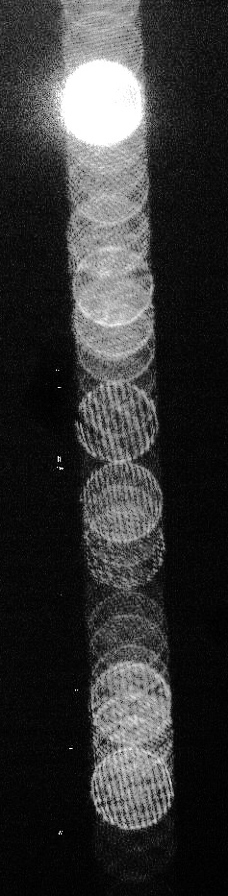
\includegraphics[height=0.6\textheight]{img/dots_cropped.jpg}
        \caption{}
    \end{subfigure}
    \begin{subfigure}[b]{0.4\textwidth}
        \centering
        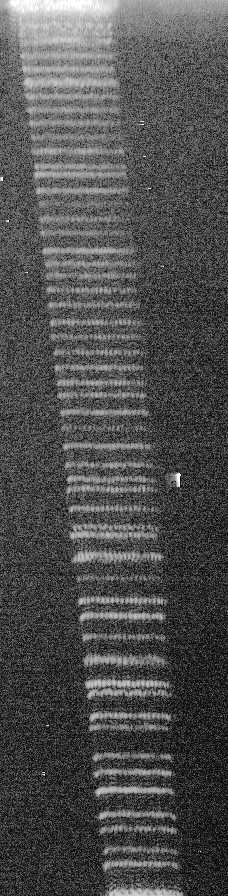
\includegraphics[height=0.6\textheight]{img/slitted.jpg}
        \caption{}
    \end{subfigure}
    \caption{Before (a) and after (b) installing the slit aperture. The aperture
    stop pares off the top and bottom halves of the defocussed circles, leaving
only a narrow center string in the middle.}
    \label{fig:globalsizing}
\end{figure}

\section{The slit aperture}
Naturally, equations \eqref{kappa} and \eqref{fringedistance-pixels} still hold.

(Insert a diagram of the setup)

(Describe how an aperture can be created in any lab)

(Show a picture of the lens with aperture)

\section{Image processing}
\label{sec:ipi-slitprocessing}
Extracting the fringe counts from such an image is straightforward. First, we
correlate the image with that of a single, solid bright rectangle which shares
the approximate dimensions of a typical strip in the image. This operation
yields intensity
peaks centered over our regions of interest. We remove closely adjacent peaks,
as they may represent questionable or overlapping strips. Compared to the sheer
number of correctly identified strips, the number of legitimate data points lost
this way is negligible. Figure \ref{fig:globalsizing-identifystrips} shows the
result of such an attempt at identifying the strips.

\begin{figure}[h]
    \centering
    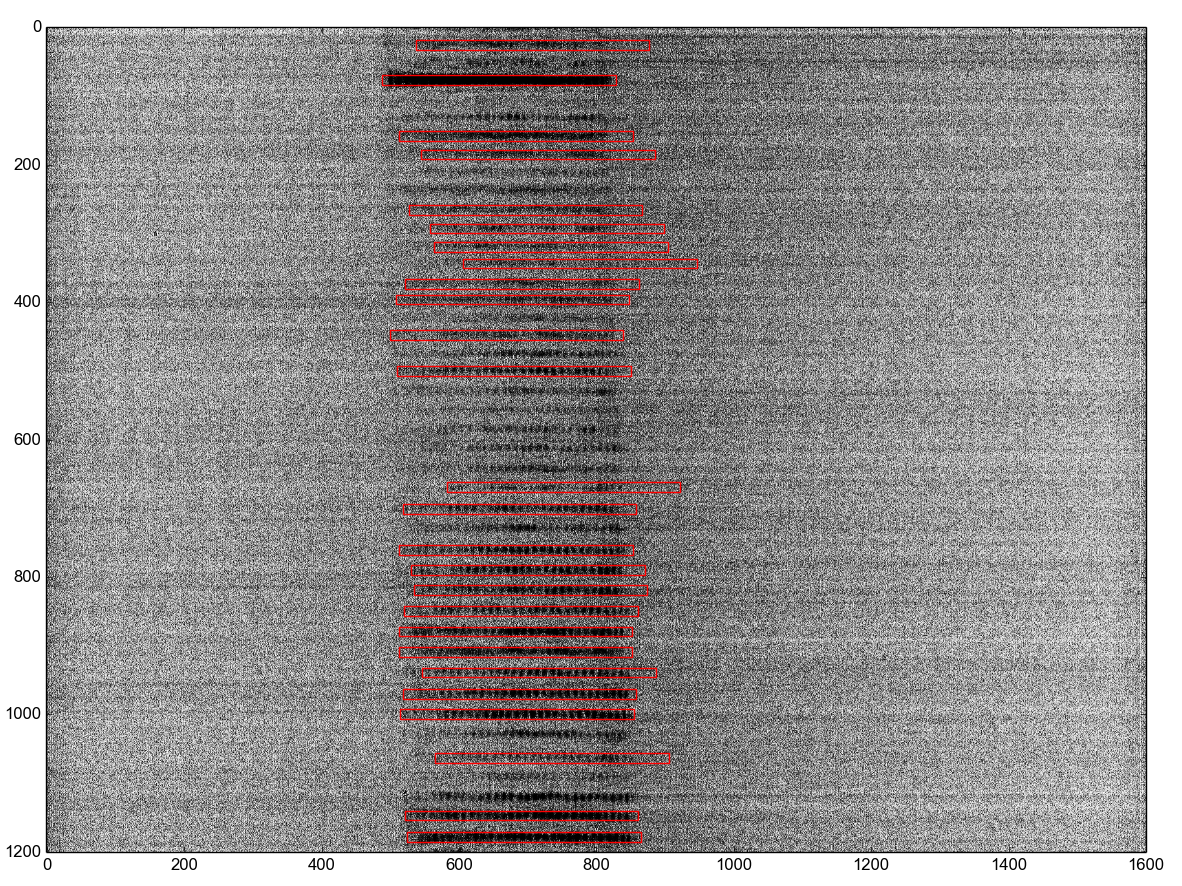
\includegraphics[height=0.38\textheight]{img/globalsizing-identifystrips.png}
    \caption{The image is correlated with that of a solid bright rectangle, which
        results in peaks that approximately coincide with the centres of the
        strips. Here, the original photo is shown with rectangles drawn centered
    at said peaks.}
    \label{fig:globalsizing-identifystrips}
\end{figure}

To find the number of fringes within the strip, we cannot rely on counting the
number of dark/bright variations directly, as some of them may be lost in the
noise. The spatial frequency of the peaks, however, taken together with the
known and constant horizontal width of the strips, will produce a reliable
fringe count. In the next step, our algorithm therefore applies the Fourier
transform to each region of interest. To improve the accuracy of the method,
three steps are performed before the Fourier transform is taken:
\begin{enumerate}
    \item a weak ($3 \times 3$) Gaussian blur is applied to the region
        (optional);
    \item a Hanning window is applied to the region -- both horizontally and
        vertically. This reduces the ``sinc ringing'' effect encountered when
        taking the Fourier transform of finite signals;
    \item the region is padded with zeros in all directions to yield a larger
        input to the Fourier transform. In our application, the windowed and padded strip
        images had dimensions of $1024 \times 1024$ pixels. Zero-padding
        increases the granularity of the frequency spectrum, which can help with
        the correct identification of the peak frequency.
\end{enumerate}

Figure \ref{fig:globalsizing-dropletpeak} shows the windowed appearance of
one such region of interest (although it does not show the padded input to the
Fourier transform due to space constraints). The Fourier transform yields a
frequency power spectrum in two dimensions, although we are primarily interested
in the frequency peak in the horizontal direction (i.e. along $y=0$). In order
to minimize the misidentification of dominant frequencies,
\begin{enumerate}
    \item we clip the spectrum to a band of reasonable frequencies. This is
        necessary because a) $1/f$-noise causes very low frequencies to dominate
        in power, although they are of no interest to us, and b) graininess in
        the original photo can sometimes result in meritless high-frequency
        peaks;
    \item we apply a Gaussian blur to the 2D spectrum to remove outliers in the
        spectrum;
    \item we discard all regions in which the peak frequency's power does not
        exceed a certain value;
    \item we discard all regions in which the \textit{prominence} of the peak
        freqency's power (i.e. its proportion to the mean power) does not exceed
        a certain value (this step is optional).
\end{enumerate}
The bottom two elements in Figure \ref{fig:globalsizing-dropletpeak} illustrate
the effect of these steps.

\begin{figure}[h]
    \centering
    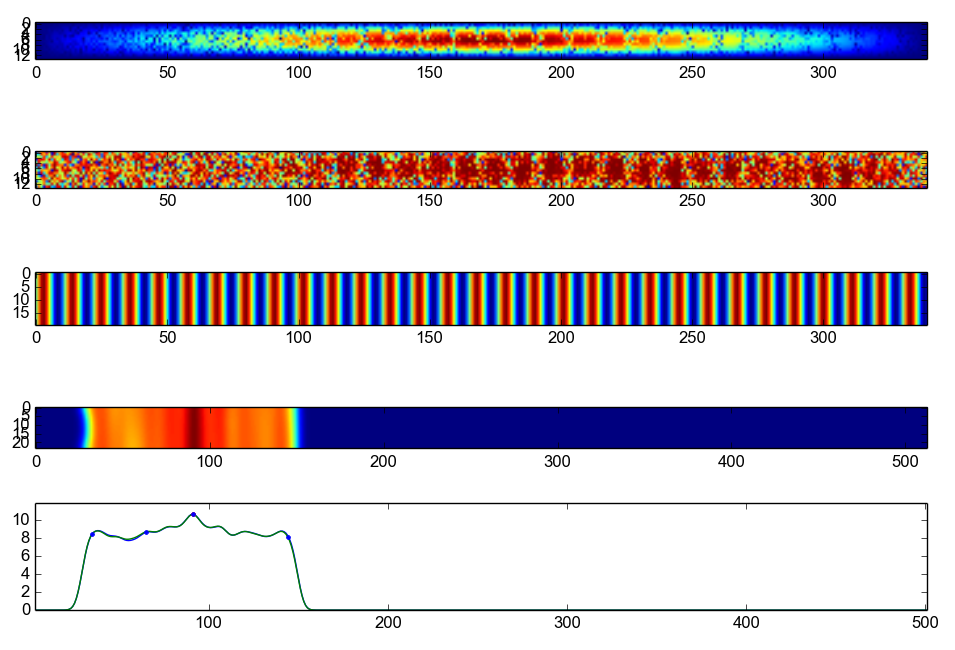
\includegraphics[height=0.38\textheight]{img/globalsizing-dropletpeak.png}
    \caption{From top to bottom: windowed region of interest; original
    (unwindowed) region of interest; sine wave representing the identified peak
frequency; clipped and lowpass-filtered 2D frequency spectrum showing a distinct
peak at about 90 oscillations across the image width of 1024 pixels; 1D plot of
the frequency spectrum, with peak identified at $f=91.0$.}
    \label{fig:globalsizing-dropletpeak}
\end{figure}

Finally, the peak frequency $f_\text{peak}$ is converted into a fringe count by re-scaling it
from the padded size $D_\text{padded}\, (= 1024$ pixels) to the width of the strip (which, in the
context of IPI measurements, should equal the diameter $D_\text{i}$ of the defocussed droplet
image):
\nomenclature{$f_\text{peak}$}{Peak frequency}
\nomenclature{$D_\text{i}$}{Diameter (in pixels) of the defocussed image}
\nomenclature{$D_\text{padded}$}{Width (in pixels) of the padded input to the
Fourier transform}
\begin{equation}
    N_\text{fr} = f_\text{peak} \frac{D_\text{i}}{D_\text{padded}}
    \label{fringes-from-diameter}
\end{equation}

In the current implementation of our algorithm, $D_\text{i}$ must be determined
and entered manually.

\section{Sources of error with the slit method}
\subsection{Misalignment of slit and lens}

While the above algorithm will generally give a good estimate of the fringe
\begin{wrapfigure}{r}{0.35\textwidth}
    \begin{center}
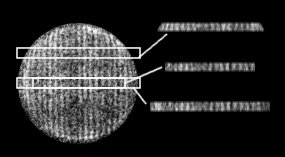
\includegraphics[width=0.33\textwidth]{img/dropletslitcropping2.jpg}
\end{center}
\caption{Only a slit aperture centered on the lens and extending across the
entire lens entrance will preserve all fringes}
\label{fig:droplet-slitcropping}
\end{wrapfigure}

count for a given defocussed droplet image, it cannot know whether the entire
center portion of the image has indeed passed the slit aperture. It is
conceivable, after all, that the slit aperture was not perfectly centered on the
lens entrance, or that the slit aperture was shorter than the diameter of the
lens entrance. Figure \ref{fig:droplet-slitcropping} illustrates how the slit
aperture can cause the defocussed image to appear smaller than it is. The
reduced value for $D_\text{i}$, manually entered in equation
\eqref{fringes-from-diameter}, will result
in droplets being reported as smaller than they are in reality.

\section{Calibrating the slit method}
Taking into account the sources of errors explained in the sections above, it is
advisable to run a few calibration tests with droplets of different sizes before
employing the IPI technique for real spray measurements. Recall that, if we
ignore the Mie error (Section \ref{sec:mie-error}), the relationship between fringe count and droplet diameter
is linear with a constant of proportionality $\kappa$ (see equation
\eqref{kappa}). The aim of our calibration, then, is to determine the value of
$\kappa$ from experiment -- the premise being that we cannot be certain of the
values of $D_a$, $z$, and possibly not even $m$ and $\phi$ (although the latter
can usually be ascertained to a sufficient degree of accuracy).

\subsection{A sample calibration of the slit aperture method}
Using the droplet generator described in Section \ref{sec:droplet-generator} and
the IPI configuration described in Section \ref{sec:ipi-setup}, we produced and
measured monodisperse droplets of many different diameters. The droplet
diameters were determined both mathematically and photographically, as described
in Section \ref{sec:verify-droplet-diameters}. Out of over 30 sets of IPI
measurements we selected six sets that exhibited both strong uniformity and
high photographic quality:

\begin{table}[h]
    \centering
    \begin{tabular}{lrrrrr}
    \toprule
    Set & Flow rate & Frequency & $D_d$, predicted  & $D_d$, from
photo & $\hat{N}_\text{fr}$ \\
    \midrule
    FA & 20.8  ml/h  & 5395 Hz  & 127 $\mu$m  & 126 $\mu$m &  9.71      \\
    FB & 39.7  ml/h  & 1990 Hz  & 220 $\mu$m  & 226 $\mu$m &  16.71     \\
    FC & 79.4  ml/h  & 1565 Hz  & 299 $\mu$m  & 291 $\mu$m &  22.92     \\
    FD & 94.3  ml/h  & 1067 Hz  & 361 $\mu$m  & 367 $\mu$m &  27.26     \\
    FE & 114.1 ml/h  & 1065 Hz  & 384 $\mu$m  & 384 $\mu$m &  29.89     \\
    FF & 175.2 ml/h  & 1038 Hz  & 447 $\mu$m  & 454 $\mu$m &  34.56     \\
    \bottomrule
\end{tabular}
\caption{Six sets of calibration data taken with the setup described in Section
\ref{sec:ipi-setup}}
\label{tab:ipi-calibration-datasets}
\end{table}
\nomenclature{$\hat{N}_\text{fr}$}{Peak fringe count measured}
The values for $\hat{N}_\text{fr}$, the peak fringe count, are based on the
histograms (see Figure \ref{fig:fringe-histograms}) showing the distribution of
fringe counts within each dataset. These fringe counts are of course found by
the algorithm described in Section \ref{sec:ipi-slitprocessing}.

It is worthwhile to point out some apparent idiosyncrasies in the histograms of
datasets FB and FC. Their peak fringe counts are 16.71 and 22.92, but there
are secondary peaks at about 21 and 29 fringes, respectively. The latter are
explained by the collision of droplets as discussed in Section
\ref{sec:droplet-collisions}, and are ignored for the purposes of calibration.

\begin{sidewaysfigure}[h!]
    \centering
    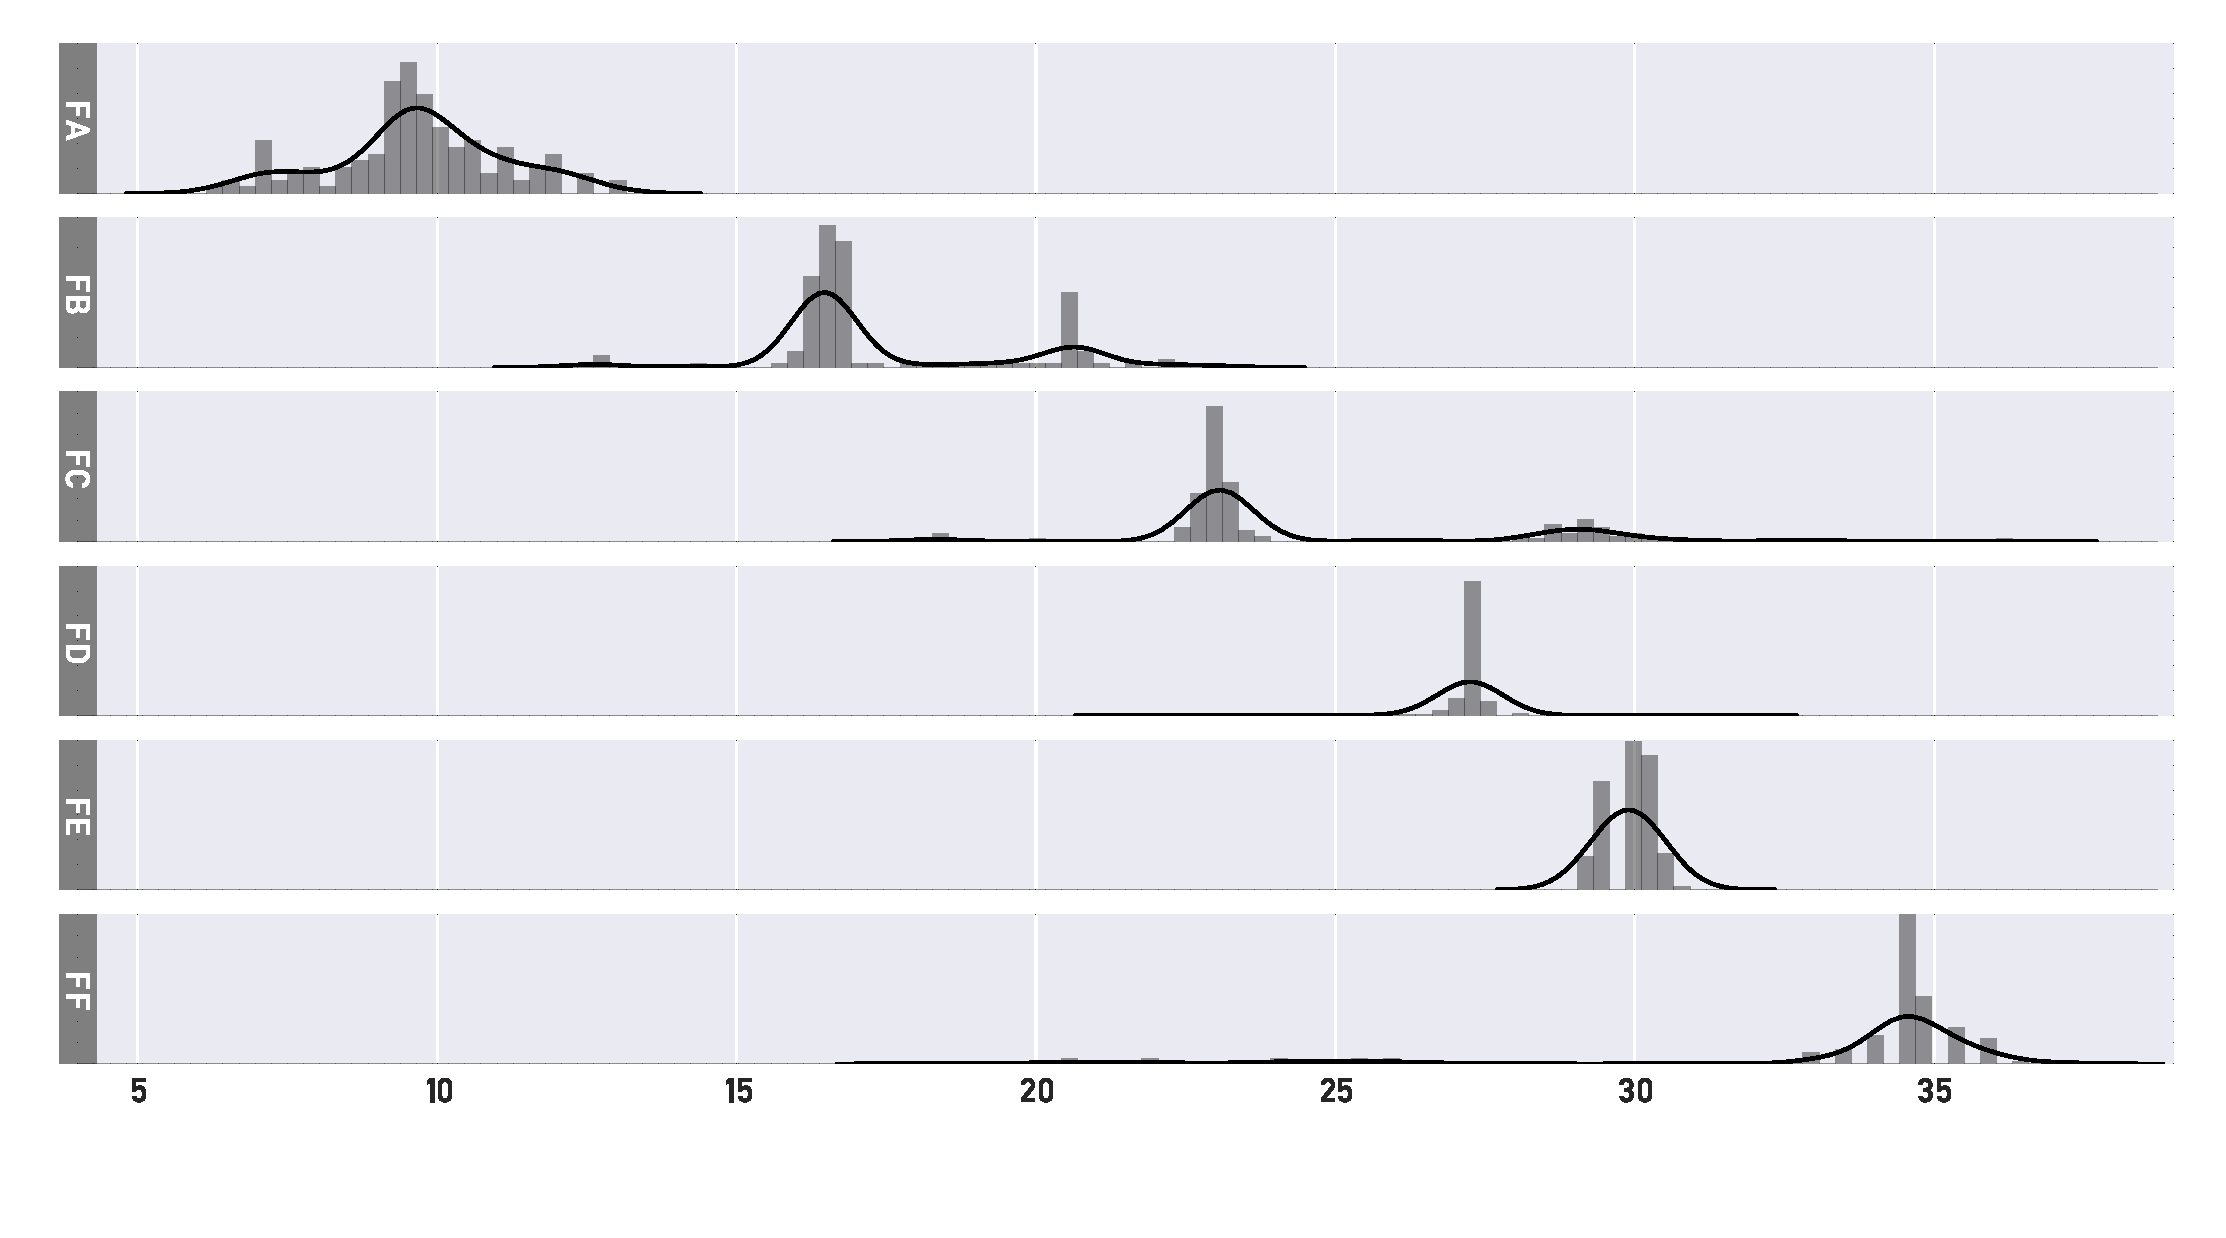
\includegraphics[width=\textwidth]{img/fringe_histogram.pdf}
    \caption{Normalized distributions of measured fringe counts $N_\text{fr}$
        for the six datasets listed in Table \ref{tab:ipi-calibration-datasets}. Solid lines are
Gaussian kernel density estimates with $h=0.5$. }
    \label{fig:fringe-histograms}
\end{sidewaysfigure}

The close agreement of the droplet diameters found from photographs with those
predicted by \eqref{berglund} reassures us that we can use the predicted $D_d$
for further analysis.

At this point, we can least-squares-fit the linear relationship \eqref{kappa} to the primary
peaks $\hat{N}_\text{fr}$ and the known droplet diameters $D_d$ to find
$\hat{\kappa}$:

\begin{equation}
    \hat{\kappa} = \frac{\sum_i D_{d,i} \, \hat{N}_{\text{fr}, i}}{\sum_i
    D_{d,i}^2}
\end{equation}

Note that instead of the standard least squares regression we here use a
simplified formula to force the trend line through the origin. This choice
should not be made lightly, since it will usually cause the residuals to have a
non-zero mean. In this case, however, we believe it to be justified to require
that $D_d = 0$ for $N_\text{fr} = 0$.

Based on the values in Table \ref{tab:ipi-calibration-datasets}, we thus arrive
at a value of $\hat{\kappa} = 76808.1$ with an $R^2$-value of 99.98\%. 

\subsection{Discussion}
Figure \ref{fig:fringe-regression} illustrates the good agreement on $\kappa$ between
all datasets. Considering the sheer number of error sources -- from the
unavoidable non-uniformity of the generated droplets to the uncertainty that
comes with taking the Fourier transform of a noisy image -- the calibration
results documented here are a testament to the practical robustness of the
method.

\begin{figure}[h!]
    \centering
    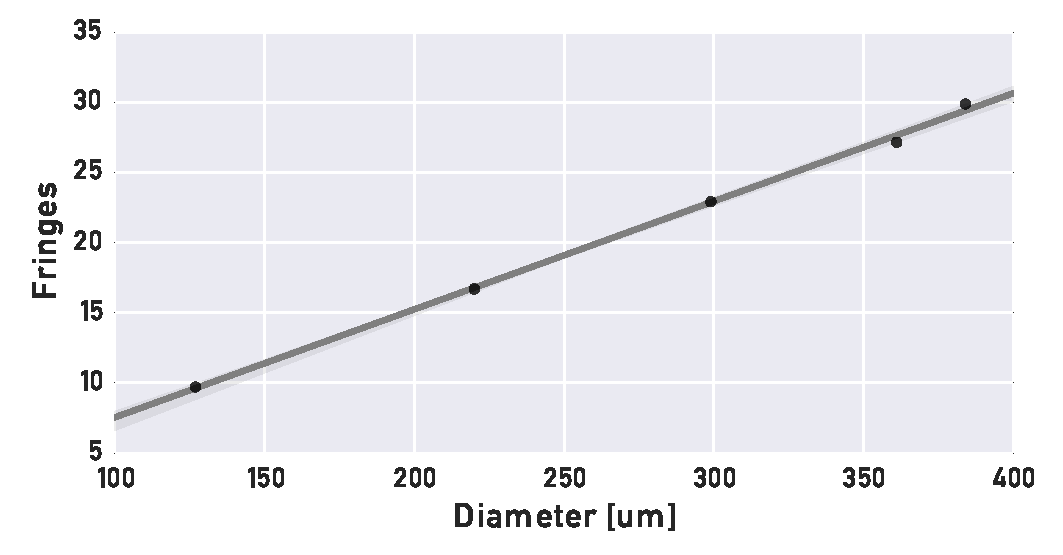
\includegraphics[width=0.8\textwidth]{img/fringe_regression.pdf}
    \caption{Scatterplot of Table \ref{tab:ipi-calibration-datasets} showing the peak fringe counts $\hat{N}_\text{fr}$ for each predicted droplet diameter $D_d$}
    \label{fig:fringe-regression}
\end{figure}
It must be remembered, of course, that the peak fringe count values
$\hat{N}_\text{fr}$ forming the basis of our calculation are taken from the
peaks of Gaussians fitted to the raw fringe count histograms (see Figure
\ref{fig:fringe-histograms}. In other words, it is our assumption that all
droplets from a given dataset produce fringe counts that are normally
distributed around their respective $\hat{N}_\text{fr}$. The histogram to
dataset FA shows a much higher deviation than the others -- this may be due to
genuine variance in the generated droplet diameters or to difficulty in
processing comparatively weak images with low fringe counts. It seems likely
that both effects contribute.

We can compare the empirically determined value $\hat{\kappa}$ with the
mathematical result obtained from \eqref{kappa}. Substituting $\lambda = 532$
nm, $m = 1.3324$ and $\phi = 90^\circ$, we conclude that
\begin{equation}
    \frac{D_a}{z} = 2 \sin \left( \frac{\hat{\kappa} \lambda}{\cos
    \frac{\phi}{2} - \frac{ m \sin \frac{\phi}{2}}{\sqrt{m^2 + 1 - 2m \cos
    \frac{\phi}{2}}}} \right) = 2\sin (3.11982 \cdot 10^{-7} \hat{\kappa})
\end{equation}
so for $\hat{\kappa} = 76808.1$, $\frac{D_a}{z} = 0.047921$. Recall that this
quotient is a measure of the collection angle and closely related to the
numerical aperture NA$=\sin \frac{D_a}{2z}$. If needed, we can now use this
result to compute the input parameters $D_a$ and $z$ in the DantecStudio IPI
software: given, for instance, $z = 45.0$ cm, we can obtain the entrace pupil
diameter as
\begin{equation}
    0.047921~\cdot~450\,\mathrm{mm} = 2.156\,\mathrm{mm}
\end{equation}


\section{Conclusion}
\begin{itemize}
    \item It's impossible to calibrate IPI using a VOAG
    \item The slit aperture works pretty well
    \item Calibration is easy, and one or two calibrations are probably enough
    \item A good collection angle (i.e. camera-laser distance) must be chosen
\end{itemize}

\chapter{Phase-Doppler\\Particle Analysis (PDPA)}

\section{Optical principle}
(Explanation)

\section{Sources of error}
\subsection{Gaussian beam divergence}
The theory predicting the linear relationship between detector phase difference
and droplet diameter is founded on the assumption of very small droplets and
plane beam wavefronts. \textbf{(Question: is it the wavefront curvature or the
non-uniformity of the intensity that causes problems?)}

The problem is termed \emph{trajectory ambiguity effect} (TAE) or \emph{Gaussian
beam defect} (GBD) in the literature.

This phenomenon was recognized first by \citet{Saffman86} but had to be neglected until
the plane-wave scattering theory of Lorenz-Mie optics was extended into
the \emph{Generalized Lorenz-Mie Theory} (GLMT). Most of this work was
done by Gouesbet, Gréhan, Maheu, Lock and others throughout the 1980s
\cite{Grehan80, Gouesbet82, Gouesbet88, Maheu88}, and mathematically
rigorous formulations were available by the early 1990s \cite{Lock94,
Gouesbet94}. The 1996 paper by Gouesbet and Gréhan summarizes these developments
and provides an early overview over the attempts to circumvent the TAE
\cite{Gouesbet96}. More discussion is given e.g. by 

Solutions are a) a planar setup, b) double-burst measurements, c) epsilon
validity measurements. It is important to align the receiver properly; the
tables used by TSI were developed using GLMT by \citet{Naqwi96}.

\subsection{Slit effect}
Durst et al show experimentally that the slit effect is even more crucial than
the Gaussian beam effect. \cite{Durst94}. Together with the TAE, this
is called the measurement volume effect. Qiu and Hsu propose using four
detectors, instead of three, to resolve this problem entirely \cite{Qiu99}. A
similar design was verified experimentally by \citet{Sipperley14}.

A more recent review of the phenomenon and associated techniques was given by
\citet{Strakey00, Strakey01}.

\subsection{Change in fringe frequency over $z$}
The curved wavefront causes the fringe spacing to vary along the axis of the
measurement volume. At the near and far ends of the volume, the fringes are
spaced wider, which can result in an error on the order of 10\%. (Red Book)

\subsection{Selection of lenses and masks}
Davis and Disimile talk about the TAE only tangentially. They provide results of
the same spray using different masks and focal lengths \cite{Davis04}.

\subsection{Optical aberrations}
See \citet{Dressler90}.

\subsection{Wrongly entered parameters}
The optical principle involves many more geometric parameters than are needed
for the operation of IPI or laser diffraction (Malvern) devices. As a result, an
excellent interface and a very attentive user are required to ensure accurate
results.

In practice, I always get error messages when doing the last step, and the
values are way out of the expected range. The result, then, is that the D20 is
made very close to the expected monodisperse diameter. Since the D20 is quite
a bit larger than the actual (and completely obvious) peak value, even these
"wrong" values aren't correct.

\section{Calibration}
Calibration is tricky, because 

knowndiam = argmax(gaussian(average(diamAB[within7percent], diamAC[within7percent])))

Since the selection of droplets with <=diff(diam) and the gaussian kernel
density estimate are one-way functions, it's impossible to work backwards. We
also want to minimize the angle in the difference-diameter plot, i.e. the PCA is
supposed to be as close as possible to 0 and 90 degrees. So the only way to do
this reliably is to iterate over the two AB and AC values to find an optimum.

Nonetheless, even with this method the relationship between the distance values
AB and AC is typically linear, and once the linear relationship has been found,
we can find the combination of values that produces the most straight PCA and
the most centered cluster. Let's approximate the 



\bibliographystyle{myplainnat}
\bibliography{bibliography}
\end{document}
